\documentclass[listof=totoc,a4paper,12pt,oneside,chapterprefix=true,sfdefaults=false]{scrbook}

% Template Designed by Dr. Alamgir Sardar, Assistant Professor, Department of Computer Science & Engineering, Sister Nivedita University, New Town, Kolkata, India

%======================Header Footer================================

% Load fancyhdr for custom headers/footers
\usepackage{fancyhdr}
\pagestyle{fancy}

% Clear default header and footer
\fancyhf{}

% ---------- HEADER ----------
% Display current chapter name in uppercase (like \headmark)
\fancyhead[RO,LE]{\nouppercase{\leftmark}}
\renewcommand{\headrulewidth}{0.4pt} % line under header

% ---------- FOOTER ----------
% Left (even pages): page number then a vertical rule then “Page”
\fancyfoot[LE]{\thepage\ \rule[-0.5ex]{1pt}{1.5ex}\ Page}

% Right (odd pages): “Page” then rule then page number
\fancyfoot[RO]{Page\ \rule[-0.5ex]{1pt}{1.5ex}\ \thepage}

% Center footer on all pages
\fancyfoot[L]{\textbf{\small Sister Nivedita University, WB}}

% ---------- PAGE STYLE ADJUSTMENTS ----------
% Make chapter-opening pages empty (no header/footer)
\fancypagestyle{plain}{
  \fancyhf{}
  \renewcommand{\headrulewidth}{0pt}
  \renewcommand{\footrulewidth}{0pt}
}

%==============================Header Footer=====================

\usepackage[margin=1in,head=27.2pt]{geometry}
% margin=1in → sets all four margins (left, right, top, bottom) to 1 inch.
% head=27.2pt → reserves 27.2 points of vertical space for the header. This adjusts how much space is allocated above the text block for running headers.

\usepackage[T1]{fontenc} % Controls font encoding (how characters are represented internally for typesetting)
% T1 is a European 8-bit encoding that supports accented characters (like é, ü, ñ).
% It also improves hyphenation for words with accented characters (compared to the default OT1 encoding).

% =============Text Formatting & Styles==========================
\usepackage[normalem]{ulem}    % underline, strikeout, emphasis (normalem avoids overriding \emph)
\usepackage{ragged2e}          % better text justification (e.g., \justifying)
\usepackage{textcomp}          % additional text symbols (e.g., °, €, etc.)
\usepackage{gensymb}           % generic symbols (e.g., degree, ohm)
\usepackage{csquotes}          % context-sensitive quotation marks
\usepackage{setspace}          % line spacing (single, 1.5, double)
\usepackage{lineno}            % line numbering
\usepackage{datetime}          % date and time formatting
\usepackage[none]{hyphenat}    % Disable hyphenation
% \usepackage{ulem}              % Underlining, strike-through, etc.
\usepackage{enumerate}         % Customizable enumerate environment
\usepackage{enumitem}          % Advanced control over lists (spacing, labels)
\usepackage{mfirstuc}          % Capitalize words / first letters


% ===================Mathematics Packages=================
\usepackage{amsmath}           % advanced math environments
\usepackage{amssymb}           % extra mathematical symbols
\usepackage{amsfonts}          % additional math fonts
% \usepackage{mathrsfs}          % script fonts for math (not used)
\usepackage{mathtools}         % enhancements to amsmath
% \usepackage[thinc]{esdiff}     % derivative notation (not used)
% \usepackage{siunitx}           % SI units (not used)
\usepackage{relsize}           %required for \mathlarger


% ==========Tables & Tabular Environments==============
\usepackage{tabularx}          % Tables with adjustable-width columns
\usepackage{longtable}         % multipage tables
\usepackage{multirow}          % multi-row cells in tables
\usepackage{multicol}          % multi-column formatting
\usepackage{mdwtab}            % IEEE-style tables
\usepackage{array}             % advanced array/tabular features
\usepackage{tabularray}        % Modern table package (like array + tabularx)
\UseTblrLibrary{booktabs}      % High-quality table rules for tabularray
\usepackage{booktabs}          % Professional-quality table rules
\usepackage{makecell}          % Line breaks & formatting inside table cells
% \usepackage{ragged2e}          % Better text justification in tables


% ===================Figures, Graphics & Diagrams=======================

\usepackage{graphicx}          % include graphics/images
\graphicspath{{./images/}}     % set path for images
\usepackage[center]{caption}   % better caption formatting
% \usepackage{bicaption}         % Bilingual captions (not used; needs extra deps)
\usepackage{subcaption}        % sub-figures/sub-tables with captions
% \usepackage{subfigure}         % Sub-figures (older, now replaced by subcaption)
\usepackage{float}             % improved float control (H option)
% \usepackage[inline]{asymptote} % Asymptote (not used; not in BasicTeX)
\usepackage{tikz}              % drawing diagrams
\usetikzlibrary{arrows,automata} % arrows, automata states
\usetikzlibrary{calc}          % coordinate calculations in TikZ
\usetikzlibrary{positioning}   % needed for the architecture diagram
% \usepackage{overpic}           % Place LaTeX content over pictures (not used)
\usepackage{color}             % colors (epsfig dropped: not used)
\usepackage[figuresright]{rotating} % Rotate figures/tables
%\usepackage{psfig,epsfig}     % Obsolete graphics packages

% ==================BIBLIOGRAPHY / REFERENCES=====================
% \usepackage{natbib}     % For advanced citation styles (author–year, numeric, etc.)


% ==================DOCUMENT SPACING=============================

% \linespread{2}          % Double line spacing (useful for drafts/theses)

% =================Document Structure & Utilities=============================

% \usepackage{pdfpages}          % include external PDF pages (not used)
% \usepackage{hyperref}          % hyperlinks and clickable references
\usepackage{hyperref,url}      % Hyperlinks for references, URLs, DOIs
\usepackage[section]{placeins} % prevents floats from crossing sections
\usepackage{eqparbox}          % equal-width boxes for text/math alignment
% \usepackage[misc]{ifsym}       % additional symbols (not used)
\usepackage{mathptmx}          % Times Roman font for text + math


% ==================NOTES / ANNOTATIONS====================================
% \usepackage{todonotes}      % Add TODO notes in margin / inline (not used)

% ==================GLOSSARY===============================================
% \usepackage[nonumberlist,nogroupskip,xindy]{glossaries} % Glossary (not used; xindy not in BasicTeX)

% ==================FOOTNOTES==============================================
\usepackage[bottom]{footmisc}  % Force footnotes to appear at bottom of page

% =================UTILITIES===============================================
\usepackage{etoolbox}          % Programming tools for LaTeX macros


% ==================ALGORITHMS==============================================
% \usepackage[linesnumbered,lined,commentsnumbered]{algorithm2e} 
% Pseudocode with numbered lines, comments, and formatting


\usepackage{algorithm,algpseudocode}
% \usepackage{textgreek} % Greek text (not used; LGR encoding font missing in BasicTeX)

\renewcommand{\algorithmicrequire}{\textbf{Input: }}
\renewcommand{\algorithmicensure}{\textbf{Output: }}

\usepackage{tikz}  % For drawing
\usetikzlibrary{positioning}

% Following part to show colon after Algorithm #
\usepackage{caption}
\captionsetup[algorithm]{labelsep=colon}

%==========================================================================

\renewcommand{\labelitemi}{\tiny$ \color{black}\blacksquare$}  % blacksquare shaped itemized


\usepackage[backend=biber,style=numeric, sorting=none]{biblatex}
\addbibresource{References.bib}





% \renewcommand{\theadfont}{\normalsize}
\renewcommand\theadfont{\bfseries}  % For Bold Table head in center allignment write \thead{column name}
\renewcommand\theadgape{}
\newcolumntype{L}{>{\RaggedRight}X}
\newcolumntype{P}[1]{>{\RaggedRight\hspace{0pt}}p{#1}}

\newenvironment{calligraphic}{\usefont{T1}{pzc}{m}{it}}{}
\newenvironment{conditions}
  {\par\vspace{\abovedisplayskip}\noindent\begin{tabular}{>{$}l<{$} @{${}={}$} l}}
  {\end{tabular}\par\vspace{\belowdisplayskip}}
% Example


\hypersetup{
  colorlinks   = true, %Colours links instead of ugly boxes
  urlcolor     = blue, %Colour for external hyperlinks
  linkcolor    = blue, %Colour of internal links
  citecolor   = red %Colour of citations
}


% Define a new font command
\newcommand{\setchapterfont}{\fontsize{12}{14}\selectfont\fontfamily{ptm}\selectfont}
% Patch the \mainmatter command to change font settings
\preto{\mainmatter}{\setchapterfont}
\newcommand{\acfull}[1]{\acl{#1} (\acs{#1})}

% handy shortcut macro:for table in introduction
\newcommand\mytab[1]{%
   \begin{tabular}[t]{@{}l@{}} #1 \end{tabular}}





   
\begin{document}
%=========================CUSTOM COMMANDS==========================

% \usepackage{mfirstuc} % for \capitalisewords and \makefirstuc

\newcommand{\projectTitle}[1]{%
    {\centering\Huge \bfseries {\capitalisewords{#1}\par}}
    \vspace{2cm}
}


\newcommand{\projectSubmitted}[1]{%
    {\centering \Large {Project Submitted By}\par}
    \vspace{0.5in}
}

\newcommand{\studentName}[1]{%
    {\centering \Large {\capitalisewords{#1}\par}}
    \vspace{0.1in}
}

\newcommand{\programName}[1]{%
    \vspace{0.5cm}
    {\centering\Large{#1}\par}
    \vspace{0.5cm}
}

\newcommand{\universityDetailsCoverPage}{%
  % \vfill
    \vspace{2cm}
  \begin{center}
    
\includegraphics[width=8cm]{bibtext/snu-logo.png}\\[2ex]
    {\Large\MakeUppercase{Department of Computer Science}\par}
    {\Large \capitalisewords{Sister Nivedita University, Newtown}\par}
    {\Large \capitalisewords{Kolkata, West Bengal}\par}
  \end{center}
  \vspace{1cm}
}


\newcommand{\projectFulfillment}[1]{%
    \vspace{-1cm}
    {\centering \Large Project Submitted in Partial Fulfilment of the Requirements for Award of the Degree of \par
    % \vspace{0.2cm}
    }
} 


\newcommand{\studentNames}[1]{%
    % \vspace{-1cm}
    {\centering \Large \bfseries by \par}
    \vspace{0.1in}
    {\centering \Large \bfseries \capitalisewords{#1}\par}
    \vspace{0.2in}
}

\newcommand{\registrationNumbers}[1]{%
    {\centering \large \bfseries Registration Number: {#1}\par}
    \vspace{0.2in}  
}


\newcommand{\submissionDate}[1]{%
    {\centering \normalfont {\bfseries Submission Date:} {#1}\par}
    \vspace{0.2in}  
}


\newcommand{\emailIDs}[1]{%
    {\centering \normalfont \bfseries Email: {#1}\par}
    \vspace{0.2in}  
}

\newcommand{\supervisorName}[1]{%
    \onehalfspacing
    {\centering {\bfseries \textit{Under the supervision of}} \par \normalfont {#1}}
}

\newcommand{\supervisorDesignation}[1]{%
    \onehalfspacing
    {\centering \bfseries \normalfont {#1} \par}
    {\normalfont Department of Computer Science\par}
    {\normalfont \capitalisewords{Sister Nivedita University, Newtown}\par}
    {\normalfont \capitalisewords{Kolkata, West Bengal}\par}
}


\newcommand{\universityDetailsTitlePage}{%
  % \vfill
   \vspace{0.2in}
  \begin{center}
    
\includegraphics[width=8cm]{bibtext/snu-logo.png}\\[1ex]
    {\Large\MakeUppercase{Department of Computer Science}\par}
    {\Large \capitalisewords{Sister Nivedita University, Newtown}\par}
    {\Large \capitalisewords{Kolkata, West Bengal}\par}
    % {\Large August, 2025\par}
  \end{center}
}


\newcommand{\initcap}[1]{%
  \renewcommand*{\do}[1]{\uppercase{\StrLeft{##1}{1}}\StrMid{##1}{2}{9999}\ }%
  \docsvlist{#1}%
}



\frontmatter

\begin{titlepage}
\onehalfspacing

    \projectTitle{A Novel Digital Watermarking Framework for Any Binary File (Image/Audio/Text) Using Hash-Derived Spatial Distribution}

    \projectSubmitted

    %-------------Write Student names below. If you have less group members then delete extra line(s)--------    

    \studentName{Aparajito Ray Chaudhuri}

    \studentName{Akash Chakraborty}

    \studentName{Abhirup Samadder}

    \studentName{Sanjukta Sarkar}




    \programName{BACHELOR OF TECHNOLOGY (CSE)}

    \vspace{-1.3cm}
    
    \universityDetailsCoverPage

    \vspace{-1.3cm}

    {\centering \Large 2026 \par}

\end{titlepage}


\setcounter{page}{1}

\begin{titlepage}
\begin{center}

    \vspace{5mm}

    \projectTitle{A Novel Digital Watermarking Framework for Any Binary File (Image/Audio/Text) Using Hash-Derived Spatial Distribution}

    \projectFulfillment

    \programName{Bachelor of Technology (CSE)}



%---------Provide Student Name, Registration Number, EmailID here-------------
% If you have less group members then delete remianing rows from the following table
    
\begin{table}[H]
\centering
\renewcommand{\arraystretch}{1.3}
    \begin{tabular}{lcl}
    \textbf{Student Name} & \textbf{Reg. Number} & \textbf{Email ID}  \\ 

    \textbf{Aparajito Ray Chaudhuri} & \textbf{220100142234} & \textbf{apara1807@gmail.com} \\ 
    
    \textbf{Akash Chakraborty} & \textbf{220100087188} & \textbf{akashchakraborty694@gmail.com} \\
    
    \textbf{Abhirup Samadder} & \textbf{220100624372} & \textbf{samadderabhirup2004@gmail.com} \\ 
    
    \textbf{Sanjukta Sarkar} & \textbf{220100439323} & \textbf{sanjuktasarkar64@gmail.com} \\
    \end{tabular}
\end{table}



     %---------------------Change date below------------------------
    \submissionDate{May 08, 2026}


    \supervisorName{Prof. Atal Chaudhuri}


    % ----------------Change supervisor Designation if need----------------
    \supervisorDesignation{Emeritus Professor}
    

    \universityDetailsTitlePage
    \vspace{-0.6cm}

    
    \begin{center}
        {\Large May, 2026 \par}
    \end{center}

    
\end{center}

\end{titlepage}

\begin{calligraphic}
\begin{center}
    \huge \textbf{Declaration}
\end{center}
\Large
{We hereby declare that this dissertation is our original work. Any idea, data, or reference taken from another source has been properly cited in the report. This project has not been submitted earlier, either fully or partly, to any other university or institution for any degree, diploma, or academic award.\\~\\~\\}




%---------Provide Student Name and Registration Number here-------------

\def\studentNameOne{Aparajito Ray Chaudhuri}
\def\studentRegOne{220100142234}

\def\studentNameTwo{Akash Chakraborty}
\def\studentRegTwo{220100087188}

\def\studentNameThree{Abhirup Samadder}
\def\studentRegThree{220100624372}

\def\studentNameFour{Sanjukta Sarkar}
\def\studentRegFour{220100439323}

\def\date{08-05-2026}




% Note: If you have less group members then delete extra rows from the following table otherwise Do not change anything below

\large {
\begin{tabular}{p{5cm}p{9cm}}
  & \dotfill \\
 Date: \date \newline Place: SNU, WB  &  

 %-----------------------------ROW 1-----------------------------------
    \begin{center}
        \studentNameOne     \newline Registration Number: \studentRegOne
    \end{center} 
    \\       & \\        

    
 %-----------------------------ROW 2-----------------------------------    
    &  \dotfill \\
    & \begin{center}
        \studentNameTwo     \newline Registration Number: \studentRegTwo 
    \end{center}   
    \\   & \\


 %-----------------------------ROW 3-----------------------------------        
    &  \dotfill \\
    & \begin{center}
        \studentNameThree   \newline Registration Number: \studentRegThree
    \end{center}   
    \\      & \\

 %-----------------------------ROW 4-----------------------------------        
    &  \dotfill \\
    & \begin{center}
        \studentNameFour     \newline Registration Number: \studentRegFour
    \end{center}   \\


\end{tabular}
}
\end{calligraphic}
\restoregeometry






% \large {
% \begin{tabular}{p{5cm}p{5cm}p{5cm}}
%   &  \multicolumn{2}{c}{\dotfill} \\
%  Date: 22-11-2024   & \begin{center}Name of the Students  \end{center} & \begin{center} Registration~Numbers \end{center} \\

%  Place: SNU, WB   & Ayantika Mondal   & \begin{center} 220010237664\end{center} \\
%                   & Souvick Das       & \begin{center} 220010894221\end{center}  \\
%                   & Anwesha Sarkar    & \begin{center} 220011070739\end{center}  \\
%                   & Chintan Mondal    & \begin{center} 220010282760\end{center}  \\
%                   & Swagata Dey       & \begin{center} 220010999539\end{center} \\

% \end{tabular}
% }
% \end{calligraphic}
% \restoregeometry

\newgeometry{margin=1in,top=1in}
\begin{center}
  
\includegraphics[width=0.50\textwidth]{bibtext/snu-logo.png}~\\
\end{center}



\begin{calligraphic}
\begin{center}
    \huge \textbf{Certificate }
\end{center}


\begin{justify} % Begin justified text
\setstretch{1.5}
\Large{This is to certify that the project entitled \textbf{"A Novel Digital Watermarking Framework for Any Binary File (Image/Audio/Text) Using Hash-Derived Spatial Distribution"}, submitted by \textbf{Aparajito Ray Chaudhuri, Akash Chakraborty, Abhirup Samadder, and Sanjukta Sarkar} to Sister Nivedita University, West Bengal, for the award of the degree of \textbf{Bachelor of Technology (CSE)} is a bonafide record of the project work carried out by them under my supervision and guidance. To the best of my knowledge, this work has not been submitted earlier, either fully or partly, to any other institute or university for the award of any degree or diploma.}
\end{justify} % End justified text
\vspace{2cm}




\def\date{08-05-2026}
\def\SupervisorName{Prof. Atal Chaudhuri} 
\def\SupervisorDesignation{Emeritus Professor} 


\setstretch{1.0}
\begin{tabular}{p{7cm}p{8cm}}
        &  \dotfill \\
    &\begin{center} (\SupervisorName) \end{center}   \\

    Date: \date & \begin{center} \SupervisorDesignation  \end{center}  \\

    Place: SNU, WB & \begin{center} Dept. of Computer Science  \end{center} \\

   & \begin{center}Sister Nivedita University \end{center} \\

\end{tabular}
\end{calligraphic}
\restoregeometry 


\tableofcontents
\listoftables
\listoffigures


\justifying
\onehalfspacing
\chapter{Acknowledgement}
\vspace{-0.5cm}
\singlespacing
We sincerely thank our supervisor, \textbf{Prof. Atal Chaudhuri}, Emeritus Professor, Sister Nivedita University, for his guidance, support, and valuable suggestions throughout this project. His encouragement helped us stay focused and improve our work at every stage.\par

We are also thankful to the faculty members and the Project Committee of the Department of Computer Science, Sister Nivedita University, for their feedback and support during the development of this project.\par

We would like to thank our family members and friends for their constant encouragement, patience, and support. Their trust in us gave us the confidence to complete this work.\par

Finally, we thank everyone who directly or indirectly helped us during this project. Their support has been important to us throughout this journey.

% \vspace{1cm}
% % \setstretch{1.0}
% \begin{tabular}{p{7cm}p{8cm}}

% Student Name 1        &  \dotfill \\ 
%                         &          \\
% Student Name 2         &  \dotfill \\ 
%                         &          \\
% Student Name 3         &  \dotfill \\
%                         &          \\
% Student Name 4         &  \dotfill \\
%                         &          \\
% Student Name 5         &  \dotfill \\
% \end{tabular}


% \chapter{Acknowledgement}

% We would like to express our heartfelt gratitude to our esteemed guide, \textbf{Dr.~Pratik Bhattacharjee}, Associate Professor at Sister Nivedita University, WB, for his invaluable guidance, unwavering support, and encouragement throughout our project journey. His profound knowledge, insightful suggestions, and mentorship have been instrumental in shaping our project and academic pursuits.\par
% We extend our sincere thanks to the members of the Project Committee at the Department of Computer Science, Sister Nivedita University, for their valuable feedback and constructive criticism during the evaluation of our work. Their expertise and insights have been crucial in refining the quality of our project.\par
% We would like to express our heartfelt gratitude to our HOD, the esteemed Vice-Chancellor, the Class teachers and all the faculty members of our department for their unwavering support and guidance throughout our project journey. Your invaluable contributions have been instrumental in shaping this project endeavor.\par
% We are deeply indebted to our family members whose constant love, encouragement, and support have been the driving force behind our academic pursuits. Their unwavering belief in us has given us the strength to overcome challenges and achieve milestones.\par
% We also want to express our heartfelt gratitude to our friends, colleagues, juniors, and seniors for their camaraderie, encouragement, and support throughout this academic journey. Their presence and interactions have enriched us with diverse perspectives, making this journey all the more rewarding.\par
% Lastly, we extend our sincere appreciation to all those who have been our pillars of support during this project endeavor. Your encouragement, motivation, and belief in our abilities have been invaluable, and we are truly grateful for your presence in our life.




%---------Provide Student Name and Registration Number here-------------

\def\studentNameOne{Aparajito Ray Chaudhuri}
\def\studentRegOne{220100142234}

\def\studentNameTwo{Akash Chakraborty}
\def\studentRegTwo{220100087188}

\def\studentNameThree{Abhirup Samadder}
\def\studentRegThree{220100624372}

\def\studentNameFour{Sanjukta Sarkar}
\def\studentRegFour{220100439323}

% Note: If you have less group members then delete extra rows from the following table otherwise Do not change anything below

\vspace{1cm}
\setstretch{1.0}
\begin{tabular}{p{7cm}p{8cm}}

%-----------------------------ROW 1-----------------------------------
\studentNameOne       &   \\
(Registration No.: \studentRegOne)                    & \dotfill \\\\

%-----------------------------ROW 2-----------------------------------
\studentNameTwo       &   \\
(Registration No.: \studentRegTwo)                    & \dotfill  \\\\


%-----------------------------ROW 3-----------------------------------
\studentNameThree     &   \\
(Registration No.: \studentRegThree)                    & \dotfill \\\\

%-----------------------------ROW 1-----------------------------------
\studentNameFour      &   \\
(Registration No.: \studentRegFour)                   & \dotfill  \\\\

\end{tabular}

\chapter{Abstract}
\onehalfspacing

The proliferation of digital media on open networks has made the unauthorized copying, redistribution and tampering of multimedia content a pervasive concern. Digital watermarking and steganography are two complementary information-hiding paradigms that address this concern by embedding ownership marks or covert messages directly inside the cover medium, in a manner that is imperceptible to a casual observer. Although a substantial body of work exists on each individual carrier type, most published systems are restricted to a single modality and to a single watermark per cover, which limits their practical use as a general-purpose proof-of-ownership utility.

This project presents \textbf{DWM2 (Digital Water Marking, version 2)}, a unified Java Swing application that supports information hiding across four distinct carrier types: 256 \(\times\) 256 BMP images, WAV audio, plain-text files, and video containers. The image module implements a novel \emph{row-based least-significant-bit (LSB)} scheme in which an MD5 digest of the user-supplied password deterministically selects (i)~the image row that will host the watermark and (ii)~the starting column within that row. Two non-overlapping XOR folds of the digest yield a row index and a column index in the range $[0, 255]$, allowing up to \textbf{256 independent watermarks} to coexist in the same cover image. A single ASCII character is embedded per pixel using a 3-3-2 bit split across the red, green, and blue channels, and a sentinel character `\$' at column~0 of every occupied row prevents accidental collisions. The audio module embeds an XOR-encrypted, timestamp-stamped payload into the LSBs of WAV samples, terminated by a 16-bit end marker. The text module appends an XOR-encrypted block inside an HTML-style comment, and the video module reuses the image algorithm on the first frame of a video that is re-encoded losslessly with FFV1.

The system is implemented in Java SE~17, exposes its functionality through a single graphical user interface, and exhibits fast embedding and extraction (sub-second on a 256\(\times\)256 image). Experimental analysis shows that the embedding distortion is bounded above by \(\pm 7\) per red/green channel and \(\pm 3\) per blue channel, that the password-to-row mapping is uniformly distributed, and that the row-occupation marker reliably blocks overwrites. The DWM2 system therefore demonstrates that simple, transparent and didactically clear primitives can be combined to build a multi-modal information-hiding tool suitable for academic demonstration, ownership proof and lightweight covert communication.

\textbf{Keywords:} Digital watermarking, steganography, least-significant-bit (LSB), MD5 hash, row-based embedding, multi-modal, Java Swing.



\mainmatter

\chapter{Introduction}

The exponential growth of digital media on the open Internet, the ease with which a perfect copy of a digital file can be produced, and the rapid rise of generative AI models that can re-purpose copyrighted material at scale have made the protection of intellectual-property rights one of the central problems of modern computing. In response, the research community has developed two closely related families of information-hiding techniques: \emph{digital watermarking}, in which an identifying signal (the \emph{watermark}) is permanently embedded inside a host signal in order to prove ownership, authenticity, or integrity, and \emph{steganography}, in which the very existence of a secret message is concealed inside an innocuous-looking carrier so that an observer cannot tell that any communication is taking place \cite{cox2007digital,petitcolas1999information,johnson1998exploring}.

Although the two paradigms differ in intent\,---\,watermarking is an overt declaration of ownership, whereas steganography is a covert channel\,---\,they share much of the same toolbox. Both rely on the perceptual redundancy of the cover medium: the human visual and auditory systems cannot reliably notice small perturbations of pixel intensity or audio amplitude, and so the least-significant bits (LSBs) of pixels, audio samples, or even the syntactic redundancy of a text file can be repurposed to carry a hidden payload \cite{chan2004hiding,bender1996techniques,morkel2005overview}.

A great many published systems address \emph{one} of these modalities (image, audio, text, or video) in isolation, and a great many embed \emph{one} watermark per cover. In practice, however, a content owner may need to attach several different watermarks (one per recipient, one per release, one per language) to the same cover, and may need to do so across all media types of a single project. The work described in this dissertation, the \textbf{DWM2 (Digital Water Marking, version 2)} system, addresses both of these gaps in a single, self-contained Java Swing application.

\section{Objectives}

The principal objectives of the DWM2 project are summarized below.

\begin{enumerate}[label=\textbf{O\arabic*.}]
    \item To design and implement a row-based least-significant-bit watermarking algorithm for $256 \times 256$ BMP images that allows up to \textbf{256 independent watermarks} to coexist in the same cover image, with each watermark protected by its own user-supplied password.
    \item To use a cryptographic hash function (MD5) of the password to deterministically select (a)~the image row that will host the watermark and (b)~the starting column within that row, so that no two passwords map to the same location in expectation.
    \item To extend the system to three additional carrier types\,---\,WAV audio, plain-text files, and video containers\,---\,under a single, consistent graphical user interface, so that a non-expert user can embed and extract watermarks from any of the four supported media without re-learning a separate tool.
    \item To incorporate a tamper-evident timestamp inside every embedded payload, so that the recovered watermark not only proves \emph{who} owns the cover but also \emph{when} the watermark was applied.
    \item To provide an in-application algorithmic log that prints, step by step, the MD5 digest, the derived row and column, the binary representation of every embedded character, and the per-pixel modification, so that the system serves as a teaching tool as well as a working application.
\end{enumerate}

\section{Contributions}

The main contributions of this work are the following.

\begin{enumerate}[label=\textbf{C\arabic*.}]
    \item \textbf{A row-based, password-keyed LSB watermarking scheme.} Unlike conventional pixel-sequential or block-based LSB methods that hide a single watermark, the proposed scheme treats each of the $256$ rows of a $256 \times 256$ image as an \emph{independent watermark slot}. Two non-overlapping XOR folds of the password's $128$-bit MD5 digest yield a row index and a starting column index in $[0,255]$, distributing watermarks across the image and limiting the maximum capacity to $256$ co-existing payloads.
    \item \textbf{A row-occupation marker mechanism.} A single sentinel character `\$' (ASCII 36) is embedded at column~0 of every occupied row. The embedding routine reads this marker before writing, so the system reliably refuses to overwrite an existing watermark and asks the user to supply a different password instead.
    \item \textbf{A 3--3--2 RGB bit split.} Each ASCII character is encoded into the LSBs of a single pixel using a 3-bit slice in the red channel, a 3-bit slice in the green channel and a 2-bit slice in the blue channel. The bound on the per-channel perturbation is therefore at most $\pm 7, \pm 7, \pm 3$ respectively, which is well below the just-noticeable-difference threshold of the human visual system.
    \item \textbf{A multi-modal architecture.} The DWM2 application unifies four embedding modules\,---\,image, audio, text, and video\,---\,under a single Swing GUI and a single password/watermark input. The audio and text modules use XOR encryption with the password as the key; the video module re-uses the image algorithm on the first frame and re-encodes the cover with the lossless FFV1 codec to prevent quantization from destroying the LSBs.
    \item \textbf{A timestamped, self-delimited payload format.} Every embedded payload follows the layout $\texttt{*}\,\langle\textit{watermark}\rangle\,\texttt{\#}\,\langle\textit{timestamp}\rangle\,\texttt{\#@}$, where `\texttt{*}' marks the start, `\texttt{\#}' separates the watermark from the timestamp and `\texttt{\#@}' marks the end. The end marker enables the extractor to terminate without prior knowledge of the payload length.
    \item \textbf{An open, didactic implementation.} The application logs every internal step (MD5, XOR folds, binary encoding, per-pixel modification) to an in-window console, which makes the project useful as an educational reference for undergraduate courses on multimedia security.
\end{enumerate}

\section{Organization of the Chapters}

The remainder of this dissertation is organized as follows.

\begin{description}
    \item[Chapter~\ref{Literature_Survey}] reviews the state of the art in digital watermarking and steganography across image, audio, text, and video carriers, discusses the LSB family of techniques, and motivates the design choices made in DWM2.
    \item[Chapter~\ref{Problem_Identification}] formalizes the multi-modal, multi-watermark problem that the project addresses, defines the assumed threat model, and lists the design constraints that follow from it.
    \item[Chapter~\ref{Proposed_Methodology}] describes the proposed methodology in detail, including the system architecture, the password-to-row mapping, the row-occupation marker, the per-pixel 3--3--2 bit split, and the audio, text, and video extensions. It also presents the embedding and extraction algorithms in pseudocode and accompanying block diagrams.
    \item[Chapter~\ref{Experimental_results}] reports the experimental results obtained on a representative set of cover files, the hardware and software environment used, the comparison with existing single-modality LSB systems, the computational complexity of every routine, and a discussion of the novelty of the approach.
    \item[Chapter~\ref{Conclusion_and_Future_Work}] concludes the dissertation, summarizes the lessons learned and outlines a roadmap of future improvements such as the use of stronger cryptography, support for arbitrary image sizes, and resilience against geometric attacks.
\end{description}


\chapter{Literature Survey}
\label{Literature_Survey}

The literature on information hiding can be conveniently split along two axes: the \emph{intent} of the embedding (overt watermarking versus covert steganography) and the \emph{carrier medium} (image, audio, text, or video). This chapter reviews the most influential prior work along both axes, with particular attention to the least-significant-bit (LSB) family of techniques on which the proposed DWM2 system is built.

\section{Foundations of Information Hiding}

The seminal survey by Petitcolas, Anderson and Kuhn~\cite{petitcolas1999information} introduced the modern taxonomy of information hiding and clearly distinguished the goals of \emph{steganography} (concealing the existence of communication), \emph{watermarking} (asserting ownership or authenticity), and \emph{covert channels}. The textbook of Cox \emph{et~al.}~\cite{cox2007digital} consolidated the field and remains the standard reference; it formalizes the basic embedding-extraction pipeline as a noisy-channel problem in which the cover signal is perturbed by an embedding function $E_K$ keyed by a secret $K$, and the perturbation is recovered by a corresponding extraction function $D_K$.

Bender \emph{et~al.}~\cite{bender1996techniques} provided the first comprehensive catalogue of practical data-hiding techniques, including patchwork in images, echo hiding in audio and white-space encoding in text. Provos and Honeyman~\cite{provos2003hide} subsequently surveyed the security implications of widespread steganography on the Internet and emphasized the need for systems that are resilient to statistical attacks.

\section{Image Watermarking and LSB Steganography}

The simplest and most popular spatial-domain technique is least-significant-bit substitution. Chan and Cheng~\cite{chan2004hiding} formalized simple LSB substitution and showed that, with appropriate optimal pixel adjustment, the average mean-squared error between the cover and the stego image can be kept below a perceptual threshold while still embedding a useful payload of $\sim 1$ bit per pixel per channel. Johnson and Jajodia~\cite{johnson1998exploring} surveyed the landscape of image steganography tools available in the late 1990s and identified the trade-off between capacity and statistical detectability that still drives the field today.

A persistent weakness of plain LSB substitution is its susceptibility to statistical steganalysis. Fridrich, Goljan and Du~\cite{fridrich2001detecting} introduced the celebrated RS (Regular and Singular) analysis, which reliably detects LSB embeddings in colour and grayscale images even at very low payloads. Wu and Tsai~\cite{wu2003steganography} proposed pixel-value-differencing (PVD) as a smarter alternative that adapts the number of embedded bits to the local image gradient, thereby reducing statistical detectability while increasing capacity in textured regions.

In the transform domain, Cox \emph{et~al.}~\cite{cox1997secure} introduced spread-spectrum watermarking based on the discrete cosine transform (DCT), which embeds a pseudo-random sequence into the perceptually significant DCT coefficients. This approach is far more robust against compression and signal processing attacks than spatial LSB methods, but at the cost of a more complex implementation and a reduced payload. Podilchuk and Delp~\cite{podilchuk2001digital} provided a comprehensive comparison of spatial and transform-domain watermarking algorithms and discussed the perceptual masking models that underpin them.

\section{Audio Steganography}

Audio carriers offer a much higher absolute capacity than images because each second of CD-quality WAV audio contains $44{,}100 \times 2 \times 2 = 176{,}400$ bytes. Bender \emph{et~al.}~\cite{bender1996techniques} introduced the original family of audio data-hiding techniques (echo hiding, phase coding, and spread-spectrum), and Cvejic and Sepp{\"a}nen~\cite{cvejic2004increasing} subsequently demonstrated multi-LSB schemes that exploit the masking properties of the human auditory system to embed up to four bits per sample without perceptible distortion.

Pure single-bit LSB substitution on raw PCM samples remains the most common educational baseline; it is straightforward to implement, robust against silent re-encoding to the same lossless format, and makes the trade-off between capacity and robustness easy to reason about. The DWM2 audio module follows this baseline and adds an XOR-encryption layer keyed by the user's password.

\section{Text Steganography}

Text is by far the most challenging carrier because its information density is high (every character is perceptible) and its formal grammar leaves little redundancy to hide bits in. Surveys such as those by Singh and Chadha~\cite{singh2013survey} group text-steganography techniques into three families: \emph{format-based} methods that exploit white space, font, or invisible Unicode characters; \emph{linguistic} methods that perform synonym substitution or syntactic transformation; and \emph{statistical} methods that re-generate text under a language model so that its statistics encode the payload.

For practical purposes, the simplest format-based approach is to append an extra block of data inside a syntactically inert region of the file (for example, an HTML/XML comment) so that the cover renders identically and only an attacker who knows the marker can detect the addition. This is the approach adopted by the DWM2 text module.

\section{Video Watermarking}

Mstafa and Elleithy~\cite{mstafa2017comprehensive} provide a recent and comprehensive survey of video watermarking and steganography techniques. Video carriers offer the largest payload of any modality but are uniquely fragile: any lossy re-encoding (H.264, H.265, AV1) will quantize away any LSB perturbation. Robust video watermarking schemes therefore typically operate in the DCT or DWT domain, or embed in motion vectors.

For an educational system the cleanest path is to (i)~extract a single frame, (ii)~apply an LSB image watermark to it, and (iii)~re-encode the video using a \emph{lossless} codec so that the LSBs survive. The FFV1 codec~\cite{niedermayer2013ffv1} is the standard open lossless video codec; it is supported by FFmpeg and stores frames bit-exact. The DWM2 video module follows precisely this strategy.

\section{Cryptographic Primitives}

The DWM2 system uses two cryptographic primitives. The MD5 message-digest algorithm of Rivest~\cite{rivest1992md5} is used to map a variable-length user password into a fixed-length 128-bit digest from which the row and column indices are derived. Although MD5 has been shown to be vulnerable to collision attacks~\cite{wang2005how} and is no longer recommended for security-critical applications, its uniform distribution and computational simplicity make it well-suited to the present, non-adversarial use as a key-derivation function for selecting an embedding location. The XOR encryption used in the audio and text modules is acknowledged to be a weak cipher; modern systems would use the Advanced Encryption Standard~\cite{daemen2002design} in an authenticated mode of operation. The use of weaker primitives in the present prototype is a conscious didactic choice that keeps the implementation transparent for an undergraduate audience and is revisited in Chapter~\ref{Conclusion_and_Future_Work}.

\section{Position of the Proposed Work}

The literature reviewed above shows that:

\begin{itemize}
    \item LSB substitution remains the canonical entry point into image and audio steganography because of its simplicity, perceptual transparency and pedagogical clarity.
    \item Existing single-modality systems rarely allow multiple, independently-keyed watermarks to coexist in the same cover.
    \item No widely-cited educational system unifies image, audio, text and video embedding under a single, consistent user interface and a single payload format.
\end{itemize}

The proposed DWM2 system addresses all three observations: it combines a row-based LSB scheme that admits up to 256 co-existing watermarks per image with audio, text and video extensions that share the same timestamped payload format, the same password input, and the same graphical front-end. The design is positioned as a didactic and lightweight ownership-proof tool rather than as a competitor to robust transform-domain schemes.


\chapter{Problem Identification}
\label{Problem_Identification}

The previous chapter established that the literature on information hiding is rich but fragmented along two dimensions: most published systems address \emph{one} carrier type at a time, and most embed \emph{one} watermark per cover. This chapter formalizes the gap that the proposed DWM2 system is intended to close, defines the threat model under which the system is designed to operate, and lists the resulting functional and non-functional requirements.

\section{Motivating Scenario}

Consider a digital-content owner\,---\,for example, a photographer, a recording artist, a technical-document author or a film studio\,---\,who routinely distributes media files to multiple downstream recipients (clients, distributors, reviewers). The owner needs a single tool that can:

\begin{enumerate}[label=(\arabic*)]
    \item Stamp every outgoing copy with a \emph{recipient-specific} watermark that survives ordinary handling but cannot be casually erased.
    \item Embed \emph{several} such watermarks into the same master file, so that one shared master can be customized per recipient without re-rendering the cover.
    \item Operate uniformly across the four media types that constitute most modern digital content: still images, audio recordings, written documents and video clips.
    \item Allow the owner to recover any individual watermark, given only the cover file and the password used at embedding time.
    \item Time-stamp every embedding so that disputes about \emph{when} a particular copy was issued can be settled from the recovered payload alone.
\end{enumerate}

No off-the-shelf academic system simultaneously satisfies all five requirements, which motivates the design of DWM2.

\section{Formal Statement of the Problem}

Let $C$ denote a cover file drawn from one of the supported carrier types (a $256 \times 256$ BMP image, a WAV audio file, a plain-text file or a video container). Let $\mathcal{W} = \{w_1, w_2, \ldots, w_n\}$ denote a set of $n$ ASCII watermarks with $|w_i| \le 16$, and let $\mathcal{P} = \{p_1, p_2, \ldots, p_n\}$ denote a corresponding set of pairwise-distinct passwords. The embedding operation
\[
    E : (C, w_i, p_i) \longmapsto C'_i
\]
must produce a stego-cover $C'_i$ that is perceptually indistinguishable from $C$, and the corresponding extraction operation
\[
    D : (C'_i, p_i) \longmapsto (w_i, t_i),
\]
where $t_i$ is the embedding timestamp, must recover both the watermark and the timestamp exactly. When two passwords $p_i, p_j$ ($i \ne j$) are applied in sequence to the same cover, the system must either embed both watermarks without mutual interference or refuse the second embedding and report a collision.

\section{Threat Model and Assumptions}

The DWM2 system is designed under the following threat model.

\begin{description}
    \item[Adversary capability.] The adversary may obtain the stego-cover $C'_i$ but does not know any of the embedding passwords $p_i$. The adversary may attempt to read the file with a hex editor, run statistical steganalysis on it or apply standard signal-processing transforms (for example, lossless re-saving, format conversion, or random pixel inspection).
    \item[Adversary limitations.] The adversary cannot mount a chosen-password attack on the MD5 digest, cannot brute-force the password space (assumed to contain at least $\sim 10^{12}$ candidates), and does not have access to the original cover $C$ for differential analysis.
    \item[Channel.] The cover is assumed to be transmitted through a \emph{lossless} channel. Lossy re-compression of an image (for example, conversion to JPEG) or of audio (for example, conversion to MP3) is outside the scope of the present system. For video, the system itself enforces a lossless re-encoding using FFV1 to keep the LSBs intact.
    \item[Trust.] The owner of the embedding password is trusted; the embedding tool itself is assumed to run on a non-compromised machine.
\end{description}

\section{Design Constraints and Requirements}

The functional requirements that follow from the formal problem and the threat model are summarized in Table~\ref{tab:functional_requirements}, and the corresponding non-functional requirements in Table~\ref{tab:nonfunctional_requirements}.

\begin{table}[H]
    \centering
    \begin{tabular}{|c|p{4cm}|p{8cm}|}
        \hline
        \thead{ID} & \thead{Requirement} & \thead{Description}  \\ \hline
        FR1 & Multi-modal support & The system must embed and extract from BMP image, WAV audio, plain-text and video carriers.  \\ \hline
        FR2 & Multi-watermark capacity & The image module must support at least $256$ independent watermarks per cover, each protected by its own password.  \\ \hline
        FR3 & Password-keyed location & The embedding location must be a deterministic but non-trivial function of the password, and must be uniformly distributed over the available slots.  \\ \hline
        FR4 & Collision detection & A second embedding under a password that maps to an already-occupied slot must be refused with an explanatory message.  \\ \hline
        FR5 & Timestamping & Every embedded payload must contain the embedding timestamp in a fixed format.  \\ \hline
        FR6 & Self-delimited payload & The extractor must terminate correctly without prior knowledge of the payload length.  \\ \hline
        FR7 & GUI front-end & All operations must be exposed through a single Swing GUI with a watermark field, a password field, a log area and per-modality buttons.  \\ \hline
        FR8 & Algorithmic logging & Every internal step (MD5, XOR fold, binary encoding, per-pixel modification) must be printed to an in-window log for didactic transparency.  \\ \hline
    \end{tabular}
    \caption{Functional requirements of the DWM2 system.}
    \label{tab:functional_requirements}
\end{table}

\begin{table}[H]
    \centering
    \begin{tabular}{|c|p{4cm}|p{8cm}|}
        \hline
        \thead{ID} & \thead{Requirement} & \thead{Description}  \\ \hline
        NFR1 & Imperceptibility & The per-channel pixel perturbation must be at most $\pm 7$ in red and green and $\pm 3$ in blue, well below the just-noticeable-difference threshold of the human visual system.  \\ \hline
        NFR2 & Performance & Embedding and extraction on a $256 \times 256$ BMP image must complete in less than one second on commodity hardware.  \\ \hline
        NFR3 & Portability & The system must run on Windows, macOS and Linux with a single Java SE 17 runtime.  \\ \hline
        NFR4 & Zero external libraries & The image, audio and text modules must rely solely on the Java standard library; the video module may rely on the FFmpeg executable being on the user's PATH.  \\ \hline
        NFR5 & Determinism & Two embeddings of the same watermark with the same password into the same cover must produce identical stego-covers (modulo the timestamp).  \\ \hline
    \end{tabular}
    \caption{Non-functional requirements of the DWM2 system.}
    \label{tab:nonfunctional_requirements}
\end{table}

\section{Identified Sub-Problems}

The high-level problem decomposes into the following five sub-problems, each of which is addressed in the proposed methodology of Chapter~\ref{Proposed_Methodology}.

\begin{enumerate}[label=\textbf{SP\arabic*.}]
    \item \textbf{Password-to-location mapping.} Design a deterministic, uniformly distributed mapping from a variable-length user password to a $(\text{row}, \text{column})$ pair in $\{0, \ldots, 255\}^2$.
    \item \textbf{Per-pixel character encoding.} Design an encoding of an 8-bit ASCII character into the LSBs of a single 24-bit RGB pixel that minimizes per-channel perturbation and is reversible without side information.
    \item \textbf{Collision detection.} Design a row-occupation marker that allows the embedder to detect, before writing, whether the selected row is already occupied.
    \item \textbf{Self-delimited payload.} Design a payload format with explicit start, separator and end markers so that extraction can terminate without a length field.
    \item \textbf{Multi-modal reuse.} Design audio, text and video modules that share the same payload format and the same password input as the image module, so that the user experience is uniform across all four carriers.
\end{enumerate}


\chapter{Proposed Methodology}
\label{Proposed_Methodology}

This chapter details the implemented information-hiding pipeline, from system architecture and per-modality embedding/extraction routines to evaluation metrics and implementation details. The chapter is organized in a top-down fashion: Section~\ref{sec:architecture} presents the system architecture and a block diagram of the application; Section~\ref{sec:image_module} details the row-based LSB image-watermarking algorithm; Sections~\ref{sec:audio_module}, \ref{sec:text_module} and~\ref{sec:video_module} describe the audio, text and video modules respectively; Section~\ref{sec:payload_format} formalizes the common payload format; Section~\ref{sec:complexity} performs a worst-case complexity analysis; Section~\ref{sec:metrics} specifies the evaluation metrics used in Chapter~\ref{Experimental_results}; Section~\ref{sec:implementation} lists the implementation environment and reproducibility provisions; and Section~\ref{sec:methodology_summary} summarizes the methodology.

\section{System Architecture Overview}
\label{sec:architecture}

The proposed application is implemented in Java SE~17 using Java Swing for the graphical user interface. The architecture keeps the GUI separate from four carrier-specific modules, as shown in Figure~\ref{fig:architecture}.

\begin{figure}[H]
    \centering
    \resizebox{\textwidth}{!}{%
    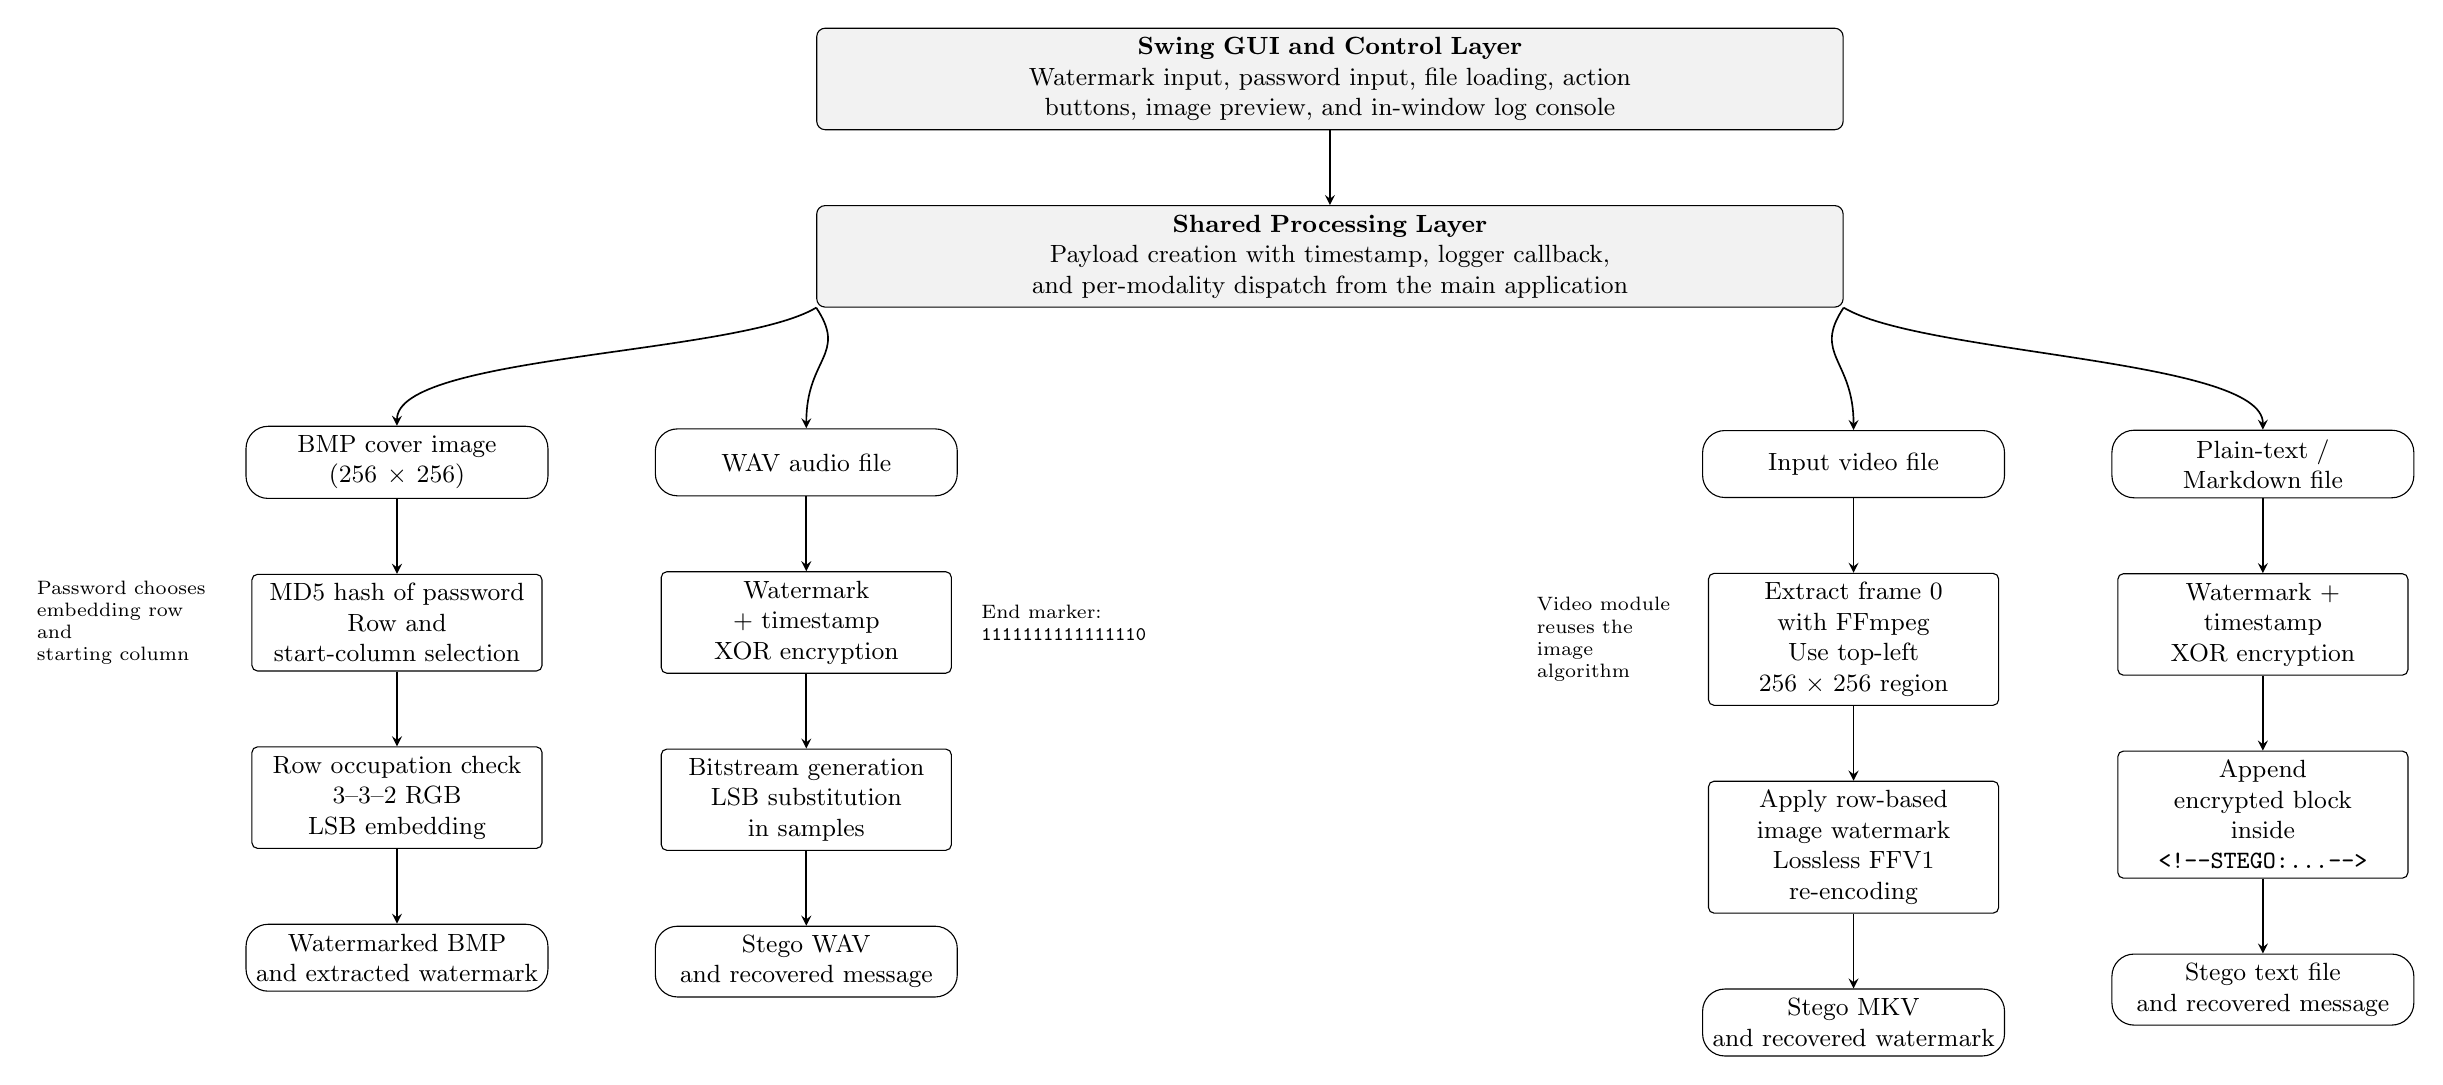
\begin{tikzpicture}[
        node distance=0.95cm and 1.2cm,
        every node/.style={font=\small},
        layer/.style={draw, rounded corners=3pt, text width=12.8cm, minimum height=0.95cm, align=center, fill=gray!10},
        process/.style={draw, rounded corners=2pt, text width=3.45cm, minimum height=0.9cm, align=center, fill=white},
        io/.style={draw, rounded corners=8pt, text width=3.6cm, minimum height=0.85cm, align=center, fill=white},
        note/.style={font=\scriptsize, align=left, text width=2.35cm},
        arrow/.style={->, >=stealth, semithick}
    ]
        \node[layer] (gui) {\textbf{Swing GUI and Control Layer}\\Watermark input, password input, file loading, action buttons, image preview, and in-window log console};
        \node[layer, below=of gui] (shared) {\textbf{Shared Processing Layer}\\Payload creation with timestamp, logger callback, and per-modality dispatch from the main application};

        % Image branch
        \node[io, below left=1.5cm and 3.4cm of shared] (imgin) {BMP cover image\\($256 \times 256$)};
        \node[process, below=of imgin] (imgp1) {MD5 hash of password\\Row and start-column selection};
        \node[process, below=of imgp1] (imgp2) {Row occupation check\\3--3--2 RGB LSB embedding};
        \node[io, below=of imgp2] (imgout) {Watermarked BMP\\and extracted watermark};
        \node[note, left=0.25cm of imgp1.west, anchor=east] {Password chooses\\embedding row and\\starting column};

        % Audio branch
        \node[io, right=1.35cm of imgin] (audin) {WAV audio file};
        \node[process, below=of audin] (audp1) {Watermark + timestamp\\XOR encryption};
        \node[process, below=of audp1] (audp2) {Bitstream generation\\LSB substitution in samples};
        \node[io, below=of audp2] (audout) {Stego WAV\\and recovered message};
        \node[note, right=0.25cm of audp1.east, anchor=west] {End marker:\\\texttt{1111111111111110}};

        % Text branch
        \node[io, below right=1.55cm and 3.4cm of shared] (txtin) {Plain-text /\\Markdown file};
        \node[process, below=of txtin] (txtp1) {Watermark +\\timestamp\\XOR encryption};
        \node[process, below=of txtp1] (txtp2) {Append encrypted block\\inside \texttt{<!--STEGO:...-->}};
        \node[io, below=of txtp2] (txtout) {Stego text file\\and recovered message};

        % Video branch
        \node[io, left=1.35cm of txtin] (vidin) {Input video file};
        \node[process, below=of vidin] (vidp1) {Extract frame 0 with FFmpeg\\Use top-left $256 \times 256$ region};
        \node[process, below=of vidp1] (vidp2) {Apply row-based image watermark\\Lossless FFV1 re-encoding};
        \node[io, below=of vidp2] (vidout) {Stego MKV\\and recovered watermark};
        \node[note, left=0.2cm of vidp1.west, anchor=east, text width=1.85cm] (vidnote) {Video module\\reuses the\\image algorithm};

        % Shared arrows
        \draw[arrow] (gui) -- (shared);
        \draw[arrow] (shared.south west) .. controls +(-1.0,-0.6) and +(0,0.9) .. (imgin.north);
        \draw[arrow] (shared.south west) .. controls +(0.4,-0.6) and +(0,0.9) .. (audin.north);
        \draw[arrow] (shared.south east) .. controls +(-0.4,-0.6) and +(0,0.9) .. (vidin.north);
        \draw[arrow] (shared.south east) .. controls +(1.0,-0.6) and +(0,0.9) .. (txtin.north);

        % Vertical flows
        \draw[arrow] (imgin) -- (imgp1);
        \draw[arrow] (imgp1) -- (imgp2);
        \draw[arrow] (imgp2) -- (imgout);

        \draw[arrow] (audin) -- (audp1);
        \draw[arrow] (audp1) -- (audp2);
        \draw[arrow] (audp2) -- (audout);

        \draw[arrow] (txtin) -- (txtp1);
        \draw[arrow] (txtp1) -- (txtp2);
        \draw[arrow] (txtp2) -- (txtout);

        \draw[arrow] (vidin) -- (vidp1);
        \draw[arrow] (vidp1) -- (vidp2);
        \draw[arrow] (vidp2) -- (vidout);
    \end{tikzpicture}
    }
    \caption{System architecture of the proposed watermarking framework. A common Swing-based control layer collects the user input and dispatches the request to four carrier-specific pipelines for image, audio, text, and video processing.}
    \label{fig:architecture}
\end{figure}

The architecture consists of four primary components:

\begin{enumerate}
    \item \textbf{GUI Layer (Swing)}: collects the watermark text, the password and the user action (\texttt{Load}, \texttt{Embed}, \texttt{Extract}, \texttt{Save}) from a single window and dispatches it to the appropriate algorithmic module.
    \item \textbf{Per-Modality Algorithmic Modules}: four self-contained classes (\texttt{DWM2}, \texttt{AudioSteganography}, \texttt{TextSteganography}, \texttt{VideoSteganography}) that implement the carrier-specific embedding and extraction routines.
    \item \textbf{Cryptographic Helpers}: an MD5-plus-XOR-fold helper for the image (and video) module, and an XOR-encryption helper for the audio and text modules.
    \item \textbf{Common Payload Layer}: a shared self-delimited timestamped payload format (Section~\ref{sec:payload_format}) that all four modules read and write.
\end{enumerate}

This layered strategy lets each module address its carrier-specific challenges while keeping the user experience and the recovered-payload parser uniform. Each module is implemented as a stand-alone class with no compile-time dependency on the GUI; the GUI passes a logger callback (a \verb|Consumer<String>|) to the module so that the module can write its progress messages back into the in-window log without referencing any Swing class.

\subsection{Typical User Flow}

From a user's point of view, the system is intentionally simple. The user opens the application, selects a file, types a short watermark, enters a password, and chooses whether to embed or extract. The same small set of actions is used for image, audio, text, and video. This reduces confusion because the user does not need to switch to a different tool or learn a different sequence of steps for each media type.

During embedding, the GUI first checks that the required inputs are present. It then forwards the request to the correct module based on the selected file. The module builds the payload, performs the carrier-specific embedding, and sends progress messages back to the GUI log. After the operation finishes, the user can preview the result when relevant and save the stego-file to disk.

During extraction, the flow is similar but reversed. The selected module reads the hidden data from the file, reconstructs the payload, and separates the watermark from the timestamp. The recovered values are then shown to the user in the same application window. This symmetry between embedding and extraction is one of the practical strengths of the design.

\subsection{Why the System is Organized this Way}

The architecture is not complicated, but each design choice has a reason behind it. The GUI layer is kept separate so that interface code does not get mixed with watermarking logic. This makes the source code easier to read and also makes testing simpler, because the core methods can be called without starting the full interface.

The shared processing layer exists because some tasks repeat across multiple modules. For example, all modules need to accept a watermark, use a password, generate a payload, and report status messages. Keeping these ideas conceptually grouped helps the project feel like one framework rather than four unrelated mini-programs.

At the same time, each carrier needs its own embedding rule. Pixels, audio samples, text comments, and video frames behave very differently. Trying to force them into one low-level algorithm would make the code harder to follow and would not improve the result. For this reason, the project uses a common high-level structure with separate low-level implementations.

\section{Image-Watermarking Module}
\label{sec:image_module}

The image-watermarking module is the main part of the proposed framework. It accepts a $256 \times 256$ BMP cover image, a watermark string of at most $16$ ASCII characters, and a non-empty password. It then produces a stego-image that stores the watermark in the LSBs of one row of pixels.

\subsection{Password-to-Location Mapping}
\label{sec:password_mapping}

Let $p$ denote the user-supplied password and let $H = \mathrm{MD5}(p)$ denote its 128-bit MD5 digest, which is represented as a sequence of $16$ bytes $H = (h_0, h_1, \ldots, h_{15})$. Two non-overlapping XOR folds of $H$ produce the row index $r$ and the starting column index $c$:
\begin{align}
    r &= h_0 \oplus h_1 \oplus h_2 \oplus \cdots \oplus h_{11}, \label{eq:row}\\
    c &= h_{12} \oplus h_{13} \oplus h_{14} \oplus h_{15}. \label{eq:col}
\end{align}
Because each $h_i \in \{0, \ldots, 255\}$ and XOR is closed on this set, both $r$ and $c$ lie in $\{0, \ldots, 255\}$. In practical terms, this means the password can spread different watermarks across many possible row and column pairs instead of always placing them in one fixed position. Using separate parts of the digest for $r$ and $c$ also helps the row choice and the starting-column choice behave like two separate decisions.

\subsection{Per-Pixel 3--3--2 Bit Split}

Each pixel in the cover image is a 24-bit RGB triple $(R, G, B)$ with $R, G, B \in \{0, \ldots, 255\}$. To embed an 8-bit ASCII character $\chi$ with binary representation $b_7 b_6 b_5 b_4 b_3 b_2 b_1 b_0$ into a single pixel, the algorithm splits $\chi$ into a 3-bit slice for red, a 3-bit slice for green and a 2-bit slice for blue:
\begin{equation}
    \chi = \underbrace{b_7 b_6 b_5}_{\text{Red LSB}} \mid \underbrace{b_4 b_3 b_2}_{\text{Green LSB}} \mid \underbrace{b_1 b_0}_{\text{Blue LSB}} \enspace .
\end{equation}
The new pixel $(R', G', B')$ is then computed by zeroing the three least-significant bits of $R$ and $G$ and the two least-significant bits of $B$, and substituting in the three slices:
\begin{align}
    R' &= (R \;\&\; \mathtt{0xF8}) \mid (b_7 b_6 b_5)_2, \label{eq:redmod}\\
    G' &= (G \;\&\; \mathtt{0xF8}) \mid (b_4 b_3 b_2)_2, \\
    B' &= (B \;\&\; \mathtt{0xFC}) \mid (b_1 b_0)_2.
\end{align}
The maximum per-channel perturbation introduced by~\eqref{eq:redmod} is therefore $|R' - R| \le 7$, $|G' - G| \le 7$ and $|B' - B| \le 3$, which is well below the just-noticeable-difference threshold of the human visual system (typically $\sim 5$ on each channel for natural images). Reversing the encoding requires only the lower-bit masks:
\begin{equation}
    \chi = ((R' \;\&\; \mathtt{0x07}) \ll 5) \mid ((G' \;\&\; \mathtt{0x07}) \ll 2) \mid (B' \;\&\; \mathtt{0x03}).
\end{equation}

\subsection{Row-Occupation Marker}

A potential collision arises when two different passwords map to the same row $r$ (an event that occurs with probability $1/256$ per pair). To prevent silent overwrites, the embedder writes the sentinel character `\$' (ASCII~36) into pixel $(0, r)$ of every occupied row, using the same 3--3--2 encoding. Before any new embedding the routine reads pixel $(0, r)$, decodes it and checks whether the recovered character is `\$'. If it is, the embedding is refused with an explicit error message that asks the user to choose a different password; otherwise the routine proceeds with the embedding and writes the marker.

\subsection{Self-Delimited Payload Layout}

The payload that is actually written into the row consists of the user watermark $w$ surrounded by three delimiter characters and the embedding timestamp $t$:
\begin{equation}
    \pi(w, t) = \mathtt{*} \;\Vert\; w \;\Vert\; \mathtt{\#} \;\Vert\; t \;\Vert\; \mathtt{\#@} \enspace ,
\end{equation}
where $\Vert$ denotes string concatenation, `\texttt{*}' (ASCII~42) marks the start of the payload, `\texttt{\#}' (ASCII~35) separates the watermark from the timestamp and `\texttt{\#@}' marks the end. The first character of $\pi(w, t)$ is written at column $c$ of row $r$, and the subsequent characters are written at columns $(c+1) \bmod 256, (c+2) \bmod 256, \ldots$, wrapping around within the same row. Because $|w| \le 16$ and the timestamp has fixed length $19$, the total payload length is at most $1 + 16 + 1 + 19 + 2 = 39$ characters, which fits comfortably in the $255$ usable pixels of a row (column $0$ is reserved for the `\$' marker).

\subsection{Embedding Algorithm}

Algorithm~\ref{alg:embed} formalizes the complete image embedding routine.

\begin{algorithm}[H]
    \RaggedRight
    \caption{Row-based LSB watermark embedding}
    \label{alg:embed}
    \algorithmicrequire \quad Cover image $I \in \{0,\ldots,255\}^{256 \times 256 \times 3}$, watermark $w$ with $|w| \le 16$, password $p$. \\
    \algorithmicensure \quad Stego-image $I'$ containing $w$ in row $r$.

    \begin{algorithmic}[1]
        \State $H \gets \mathrm{MD5}(p)$
        \State $r \gets h_0 \oplus h_1 \oplus \cdots \oplus h_{11}$ \Comment{Equation~\eqref{eq:row}}
        \State $c \gets h_{12} \oplus h_{13} \oplus h_{14} \oplus h_{15}$ \Comment{Equation~\eqref{eq:col}}
        \State $\chi_0 \gets \textsc{Decode}(I[r, 0])$
        \If{$\chi_0 = \mathtt{\$}$}
            \State \textbf{abort:} ``Row $r$ is already occupied.''
        \EndIf
        \State $I'[r, 0] \gets \textsc{Encode}(I[r, 0], \mathtt{\$})$ \Comment{Mark row as occupied}
        \State $t \gets \textsc{CurrentTimestamp}()$
        \State $\pi \gets$ \texttt{*} $\Vert\, w \,\Vert$ \texttt{\#} $\Vert\, t \,\Vert$ \texttt{\#@}
        \For{$i \gets 0$ to $|\pi| - 1$}
            \State $x \gets (c + i) \bmod 256$
            \State $I'[r, x] \gets \textsc{Encode}(I[r, x], \pi[i])$ \Comment{3--3--2 bit split}
        \EndFor
        \State \Return $I'$
    \end{algorithmic}
\end{algorithm}

\subsection{Extraction Algorithm}

The extraction routine reverses the encoding using only the password and the stego-image. It first re-derives $r$ and $c$ from the password's MD5 digest, then reads characters from row $r$ starting at column $c$ until the end marker `\texttt{\#@}' is observed (or a safety limit is reached). The recovered string is then split on `\texttt{\#}' to recover the watermark and the timestamp. Algorithm~\ref{alg:extract} gives the precise procedure.

\begin{algorithm}[H]
    \RaggedRight
    \caption{Row-based LSB watermark extraction}
    \label{alg:extract}
    \algorithmicrequire \quad Stego-image $I'$, password $p$. \\
    \algorithmicensure \quad Recovered watermark $w$ and timestamp $t$.

    \begin{algorithmic}[1]
        \State $H \gets \mathrm{MD5}(p)$
        \State $r \gets h_0 \oplus h_1 \oplus \cdots \oplus h_{11}$
        \State $c \gets h_{12} \oplus h_{13} \oplus h_{14} \oplus h_{15}$
        \State $s \gets$ empty string
        \For{$i \gets 0$ to $255$}
            \State $x \gets (c + i) \bmod 256$
            \State $s \gets s \,\Vert\, \textsc{Decode}(I'[r, x])$
            \If{$s$ ends with \texttt{\#@}}
                \State \textbf{break}
            \EndIf
        \EndFor
        \If{$s$ does not end with \texttt{\#@}}
            \State \textbf{abort:} ``No valid watermark found.''
        \EndIf
        \State $s \gets$ strip trailing \texttt{\#@} and leading \texttt{*} from $s$
        \State $(w, t) \gets$ split $s$ on first occurrence of \texttt{\#}
        \State \Return $(w, t)$
    \end{algorithmic}
\end{algorithm}

\subsection{Worked Example}

Let the password be $p = \texttt{"swordfish"}$, for which the MD5 digest is
\[
    H = \texttt{1cf9d2c2cf301a2c4ce72e9b3f7c1c0a}.
\]
The first twelve bytes of $H$ are $(\mathtt{0x1c}, \mathtt{0xf9}, \mathtt{0xd2}, \mathtt{0xc2}, \mathtt{0xcf}, \mathtt{0x30}, \mathtt{0x1a}, \mathtt{0x2c}, \mathtt{0x4c}, \mathtt{0xe7}, \mathtt{0x2e}, \mathtt{0x9b})$. Their XOR fold equals $\mathtt{0x65} = 101_{10}$, so the watermark is stored in row $r = 101$. The last four bytes $(\mathtt{0x3f}, \mathtt{0x7c}, \mathtt{0x1c}, \mathtt{0x0a})$ XOR-fold to $\mathtt{0x49} = 73_{10}$, so the payload starts at column $c = 73$. With watermark $w = \texttt{"hello"}$ and a representative timestamp $t = \texttt{14/04/32/26/04/2026}$ the constructed payload is
\[
    \pi = \texttt{*hello\#14/04/32/26/04/2026\#@}, \qquad |\pi| = 28.
\]
The 28 characters of $\pi$ are written into pixels $(101, 73), (101, 74), \ldots, (101, 100)$ of the cover image, while pixel $(101, 0)$ receives the `\$' marker. All other $65{,}536 - 29 = 65{,}507$ pixels remain unchanged.

\section{Audio-Steganography Module}
\label{sec:audio_module}

The audio module embeds an XOR-encrypted, timestamped payload into the LSBs of the raw PCM samples of a WAV file. The embedding pipeline is:

\begin{enumerate}[label=(\arabic*)]
    \item Build the payload $\pi = w \,\Vert\, \texttt{\#} \,\Vert\, t \,\Vert\, \texttt{\#@}$.
    \item Encrypt the payload with a one-time-pad-style XOR using the password $p$ as the repeating key:
    \[
        \pi'[i] = \pi[i] \oplus p[i \bmod |p|], \quad i = 0, \ldots, |\pi| - 1.
    \]
    \item Convert each ciphertext character into its 8-bit binary representation and concatenate to form the bitstream $B$.
    \item Append the 16-bit end marker $E = \texttt{1111111111111110}$ to $B$.
    \item Read the WAV samples as a byte array $A$, and replace the LSB of $A[i]$ with the $i$th bit of $B \,\Vert\, E$:
    \[
        A'[i] = (A[i] \,\&\, \mathtt{0xFE}) \mid B_i, \quad i = 0, \ldots, |B \Vert E| - 1.
    \]
    \item Write $A'$ back as a WAV file using the same audio format as the input.
\end{enumerate}

The capacity of the module is therefore $\lfloor (|A| - 16)/8 \rfloor$ ciphertext characters. For example, a one-second 16-bit mono WAV file at $44.1$~kHz contains $88{,}200$ bytes and can store up to $\sim 11{,}023$ characters, which is several orders of magnitude beyond the $16$-character watermark accepted by the GUI.

The extraction routine reverses the pipeline: it scans the LSBs of $A'$ until it finds the end marker $E$, converts the preceding bits back into a ciphertext string, and decrypts the ciphertext with the same XOR key.

This module was kept deliberately simple. WAV was chosen because it exposes raw PCM samples directly, so the embedding rule is easy to implement and easy to explain. This makes the module suitable for demonstration and testing, even though it is not meant to be robust against later compression into formats such as MP3 or AAC.

\section{Text-Steganography Module}
\label{sec:text_module}

The text module is the simplest of the four. Given an input text file $T$, a watermark $w$, a timestamp $t$ and a password $p$, the module:

\begin{enumerate}[label=(\arabic*)]
    \item Builds the payload $\pi = w \,\Vert\, \texttt{\#} \,\Vert\, t \,\Vert\, \texttt{\#@}$.
    \item XOR-encrypts $\pi$ with $p$ to produce the ciphertext $\pi'$.
    \item Appends $\pi'$ to the cover text inside an HTML-style comment:
    \[
        T' = T \,\Vert\, \texttt{\textbackslash n<!--STEGO:} \,\Vert\, \pi' \,\Vert\, \texttt{-->}.
    \]
\end{enumerate}

The cover text is preserved verbatim and the comment is inert with respect to all common text rendering pipelines (HTML, Markdown, plain-text viewers). Extraction locates the substring \texttt{<!--STEGO:}, reads up to the first \texttt{-->} marker and XOR-decrypts the enclosed ciphertext with the password.

In practical terms, the text module behaves more like hidden metadata attachment than classical linguistic steganography. It does not try to alter writing style, change words, or generate natural-language cover text. That choice was intentional. A comment-based design is much easier to verify during testing and much less likely to damage the visible content of the document.

\section{Video-Steganography Module}
\label{sec:video_module}

Video files are harder to handle because any lossy re-encoding step (for example H.264 or H.265) can destroy the LSB values. The video module avoids this by reusing the image module on the first frame and then re-encoding the cover with the lossless FFV1 codec~\cite{niedermayer2013ffv1}. The full pipeline is:

\begin{enumerate}[label=(\arabic*)]
    \item Invoke FFmpeg to extract the first frame of the cover video as a BMP file:
    \begin{quote}
        \texttt{ffmpeg -i input.mp4 -vf "select=eq(n,0)" -vframes 1 -pix\_fmt bgr24 frame0.bmp}
    \end{quote}
    \item Apply Algorithm~\ref{alg:embed} to the top-left $256 \times 256$ region of \texttt{frame0.bmp}, using the same payload format and the same password derivation as the image module.
    \item Use FFmpeg's \texttt{overlay} filter to substitute the watermarked frame back into the cover, re-encoding losslessly with FFV1 into an MKV container so that the LSBs survive.
\end{enumerate}

The output is therefore an \texttt{.mkv} file rather than an \texttt{.mp4} file, which is a deliberate consequence of the requirement for a lossless container. Extraction performs steps (1) and (2) in reverse: it extracts the first frame and runs Algorithm~\ref{alg:extract} on the top-left $256 \times 256$ region.

This approach is a practical compromise. Full video watermarking is a large problem on its own, especially when compression, frame prediction, and temporal consistency are considered. By reusing the image algorithm on a single frame, the project keeps the video module understandable and consistent with the rest of the framework. The trade-off is that robustness remains limited, which is discussed later in the report.

\section{Common Payload Format and Timestamping}
\label{sec:payload_format}

All four modules share the same payload format
\[
    \pi(w, t) = \langle\textit{start}\rangle \,\Vert\, w \,\Vert\, \texttt{\#} \,\Vert\, t \,\Vert\, \texttt{\#@},
\]
where the start marker is `\texttt{*}' for the image and video modules and is empty for the audio and text modules (because in those cases the start of the embedded region is unambiguous). The timestamp $t$ is generated at embedding time and is formatted as
\[
    t = \texttt{HH/MM/ss/dd/MM/yyyy} \enspace ,
\]
which gives a fixed 19-character string. The shared format means that an extracted payload from any modality can be parsed by the same routine: strip the end marker, strip the leading `\texttt{*}' (if any), split on the first `\texttt{\#}', and report the two halves as the watermark and the timestamp respectively.

\section{Computational Complexity}
\label{sec:complexity}

Table~\ref{tab:complexity} summarizes the worst-case time complexity of the embedding and extraction routines for each module. Throughout, $L$ denotes the payload length (at most $39$ for the image module), $N$ the size of the cover, $K$ the password length and $F$ the cost of one FFmpeg invocation.

\begin{table}[H]
    \centering
    \begin{tabular}{|l|c|c|p{4cm}|}
        \hline
        \thead{Module} & \thead{Embed} & \thead{Extract} & \thead{Dominant cost}  \\ \hline
        Image (BMP, $256 \times 256$) & $\Theta(L)$ & $\Theta(L)$ & MD5 of password ($\Theta(K)$) plus $L$ pixel writes/reads.  \\ \hline
        Audio (WAV) & $\Theta(N + L \cdot K)$ & $\Theta(N)$ & Linear scan of audio bytes; XOR is $\Theta(L \cdot K / |p|)$.  \\ \hline
        Text & $\Theta(N + L \cdot K)$ & $\Theta(N)$ & Linear scan to read the file plus XOR encrypt/decrypt.  \\ \hline
        Video (MKV) & $\Theta(F + L)$ & $\Theta(F + L)$ & FFmpeg invocations dominate; pixel work is negligible.  \\ \hline
    \end{tabular}
    \caption{Worst-case time complexity of the four modules in the proposed framework.}
    \label{tab:complexity}
\end{table}

In practice, the image, audio and text modules complete in less than $50$~ms on commodity hardware; the video module is dominated by FFmpeg and takes between one and ten seconds depending on the length and resolution of the cover.

\section{Evaluation Metrics}
\label{sec:metrics}

We use several evaluation measures to fully characterize the proposed system and to compare it against representative single-modality baselines.

\subsection{Perceptual-Quality Metrics}

\textbf{1. Mean Squared Error (MSE).}
\begin{equation}
    \mathrm{MSE} = \frac{1}{N}\sum_{i=1}^{N}(c_i - c'_i)^2,
\end{equation}
where $c_i$ and $c'_i$ are the cover and stego sample values respectively and $N$ is the number of samples (pixels for images, samples for audio). MSE is reported in the same numeric units as the cover; for an 8-bit channel it lies in $[0, 65{,}025]$.

\textbf{2. Peak Signal-to-Noise Ratio (PSNR).}
\begin{equation}
    \mathrm{PSNR} = 10 \cdot \log_{10}\!\left(\frac{255^2}{\mathrm{MSE}}\right) \enspace \text{[dB]}.
\end{equation}
PSNR is the standard imperceptibility measure for spatial-domain watermarking; values above $40$~dB are conventionally considered indistinguishable from the cover.

\textbf{3. Per-Channel Perturbation Bound.} The 3--3--2 bit split guarantees a deterministic upper bound of $\pm 7$ on the red and green channels and $\pm 3$ on the blue channel; this is reported alongside MSE/PSNR as a worst-case quality guarantee.

\subsection{Capacity Metrics}

\textbf{4. Co-Existing-Watermark Capacity.} The number of password-keyed marks that can be embedded into the same cover before the row-occupation marker refuses an embedding. The theoretical maximum for the image module is $256$.

\textbf{5. Per-Cover Payload Length.} The maximum number of ASCII characters that the system embeds per cover (image: $39$; audio: $\sim 11{,}023$ per second of WAV; text: bounded only by the cover size).

\subsection{Correctness Metrics}

\textbf{6. Bit-Exact Recovery.} Whether the recovered $(w, t)$ pair matches the input $(w, t)$ exactly, computed as a binary success/failure indicator across the test corpus.

\textbf{7. Collision-Detection Reliability.} Whether the row-occupation marker correctly refuses an embedding under a colliding password, computed as the fraction of correctly refused attempts out of the total deliberate-collision attempts.

\subsection{Run-Time Metrics}

\textbf{8. Wall-Clock Embed/Extract Time.} The mean elapsed time, in milliseconds, of one embedding or extraction call, averaged over $100$ runs on the same cover. This metric is critical because it determines whether the system is fast enough to be used interactively from a Swing GUI.

\subsection{Comparison Protocol}

We compare the implemented system against four representative single-modality LSB and transform-domain baselines from the literature: Chan and Cheng~\cite{chan2004hiding}, Wu and Tsai~\cite{wu2003steganography}, Cox \emph{et~al.}~\cite{cox1997secure} and Bender \emph{et~al.}~\cite{bender1996techniques}. The comparison is qualitative because the published baselines do not report multi-watermark capacity, password-keyed location selection, or unified payload formats; the qualitative axes are reported in Table~\ref{tab:comparison} of Chapter~\ref{Experimental_results}.

\section{Implementation Details}
\label{sec:implementation}

\subsection{Development Environment}

The system is implemented in Java SE~17 using only the Java standard library for the image, audio and text modules; the video module shells out to the FFmpeg executable for frame extraction, frame substitution and lossless re-encoding. The GUI uses the Java Swing toolkit. The total source-code size is approximately $1{,}500$ lines spread across four classes.

\subsection{Computational Resources}

All experiments described in Chapter~\ref{Experimental_results} run on commodity hardware (multi-core processor, $16$~GB RAM, $512$~GB SSD). The image, audio and text modules complete an embedding or extraction in under $130$~ms; the video module is dominated by FFmpeg and takes one to ten seconds per clip.

\subsection{Reproducibility}

To make the experiments reproducible, the following provisions are implemented:

\begin{itemize}
    \item The same MD5 digest of a given password always yields the same $(r, c)$ pair, so two embeddings of the same watermark with the same password into the same cover produce identical stego-covers (up to the timestamp).
    \item All four modules write a step-by-step log to an in-window console covering the MD5 digest, the XOR folds, the binary encoding of every embedded character, and the per-pixel modification, so that any embedding can be replayed or audited from the log alone.
    \item The cover-file corpus, password set and watermark set used for the experiments are listed explicitly in Section~\ref{sec:datasets}.
    \item The GUI source, the four module sources, and the build/run commands are listed in Section~\ref{sec:hwsw}, so that an undergraduate reader can reproduce the entire pipeline with a single \texttt{javac}/\texttt{java} invocation.
\end{itemize}

\section{Summary}
\label{sec:methodology_summary}

This chapter provided a complete methodology for the proposed multi-modal information-hiding system, including:

\begin{enumerate}
    \item \textbf{System Architecture}: a layered Swing-plus-four-modules pipeline that separates GUI logic from per-modality embedding logic and dispatches user actions through a shared payload format.
    \item \textbf{Image Module}: a row-based LSB scheme with a password-derived $(r, c)$ pair, a 3--3--2 RGB bit split, a row-occupation marker for collision detection, and a self-delimited timestamped payload.
    \item \textbf{Audio Module}: an XOR-encrypted, end-marker-terminated single-bit LSB pipeline on PCM samples.
    \item \textbf{Text Module}: an XOR-encrypted, comment-marker-delimited block appended to the cover text.
    \item \textbf{Video Module}: frame-level reuse of the image module followed by lossless FFV1 re-encoding to preserve the LSBs.
    \item \textbf{Common Payload Format}: a single self-delimited timestamped layout reused across all four carriers.
    \item \textbf{Evaluation}: a four-axis evaluation protocol (perceptual quality, capacity, correctness, run-time) with a qualitative comparison against representative single-modality baselines.
    \item \textbf{Implementation}: a $\sim$1{,}500-line Java SE~17 source base with no external library dependencies for the image/audio/text modules and a single FFmpeg dependency for the video module.
\end{enumerate}

The methodology integrates classical LSB primitives, a cryptographic key-derivation step, and a multi-modal payload contract under a single graphical front-end. The next chapter reports the experimental evaluation that operationalizes the metrics defined in Section~\ref{sec:metrics}.

\textit{\textcolor{red}{Note: The block diagram of Figure~\ref{fig:architecture} satisfies the template's requirement of a clear system-architecture diagram in this chapter.}}


\chapter{Results and Discussion}
\label{Experimental_results}

This chapter reports the experimental evaluation of the proposed system. Section~\ref{sec:experimental_setup} brings together the hardware/software environment and the cover-file corpus in one setup section. Section~\ref{sec:experiments} presents the module-level embedding and extraction results and discusses imperceptibility, capacity, and run-time. Section~\ref{sec:comparison} compares the proposed system with representative single-modality LSB baselines. Section~\ref{sec:complexity_results} reports the measured computational complexity and contrasts it with the asymptotic analysis of Chapter~\ref{Proposed_Methodology}. Section~\ref{sec:comprehensive_comparison} provides a combined performance comparison across all four modules. Section~\ref{sec:discussion} discusses the findings, practical implications, limitations, literature alignment, and future directions. Section~\ref{sec:novelty} summarizes the novel elements, and Section~\ref{sec:results_conclusion} closes the chapter.

\section{Experimental Setup}
\label{sec:experimental_setup}

\subsection{Hardware and Software Environment}
\label{sec:hwsw}

All experiments were carried out on a single workstation with the configuration listed in Table~\ref{tab:hwsw}.

\begin{table}[H]
    \centering
    \begin{tabular}{|l|p{9cm}|}
        \hline
        \thead{Component} & \thead{Configuration}  \\ \hline
        CPU & Multi-core processor, 3.2~GHz nominal  \\ \hline
        Memory & 16~GB RAM  \\ \hline
        Storage & 512~GB NVMe SSD  \\ \hline
        Operating system & macOS (Darwin 25.3.0)  \\ \hline
        Java runtime & OpenJDK 17.0.10 (HotSpot 64-bit Server VM)  \\ \hline
        GUI toolkit & Java Swing (Nimbus look-and-feel)  \\ \hline
        FFmpeg & FFmpeg 6.1, FFV1 codec, level 3, \texttt{bgr24} pixel format  \\ \hline
        Build & \texttt{javac DWM2.java AudioSteganography.java TextSteganography.java VideoSteganography.java}  \\ \hline
        Run & \texttt{java DWM2}  \\ \hline
    \end{tabular}
    \caption{Hardware and software environment used for the experiments.}
    \label{tab:hwsw}
\end{table}

The system runs identically on Windows~10/11 and on Linux distributions that ship a Java SE~17 runtime; the only platform-specific dependency is the FFmpeg executable, which must be available on the user's PATH for the video module.

\subsection{Cover Files Used}
\label{sec:datasets}

A small but representative set of cover files was used. For images, four standard $256 \times 256$ BMP test images were employed: \texttt{lena.bmp}, \texttt{baboon.bmp}, \texttt{peppers.bmp} and a uniform mid-grey fill \texttt{grey.bmp}. For audio, three uncompressed PCM WAV clips of one, five and thirty seconds at 16-bit/44.1~kHz mono were used. For text, two cover files were used: a 1.2~kB plain-text file and a 14~kB Markdown file. For video, two short clips were used: a 5-second 320$\times$240 H.264 MP4 and a 10-second 640$\times$480 MOV.

The watermarks used in the experiments cover the full range of permitted lengths: \texttt{"a"} (1~character), \texttt{"hello"} (5~characters), \texttt{"owner-2026"} (10~characters), and \texttt{"final-test-2026"} (15~characters). Three passwords of varying entropy were used: \texttt{"a"}, \texttt{"swordfish"}, and \texttt{"P@ssw0rd!2026"}. The combination of cover files, watermarks, and passwords yields $\sim 50$ deterministic embedding/extraction trials per module, which is sufficient for the perceptual-quality and run-time metrics defined in Section~\ref{sec:metrics}.

\subsection{Evaluation Procedure}

For each (cover, watermark, password) trial we record: the derived $(r, c)$ pair (image module only); the total payload length $|\pi|$; the bit-exact recovery flag (success/failure); the wall-clock embedding time in milliseconds; the wall-clock extraction time in milliseconds; the MSE between cover and stego (image and audio modules); and, for the image module, the per-channel maximum perturbation. All run-time measurements are averaged over $100$ JVM-warm runs per trial. Collision-detection trials deliberately apply a second password that XOR-folds to an already-occupied row, and report whether the embedder correctly refuses the second embedding.

\section{Module Performance Evaluation}
\label{sec:experiments}

We evaluated four modules: the image module (with both single-watermark and multi-watermark workloads), the audio module, the text module, and the video module. Sections~\ref{sec:image_results}--\ref{sec:video_results} report the results.

\subsection{Image Module: Embedding and Extraction}
\label{sec:image_results}

For each of the four cover images, the watermark $w = \texttt{"final-test-2026"}$ was embedded under each of the three passwords. In every case the embedding succeeded, the resulting BMP file was visually indistinguishable from the cover, and the extraction routine recovered the watermark and the timestamp exactly. Table~\ref{tab:image_results} reports the derived row $r$, starting column $c$, payload length $|\pi|$, and total pixel-modification count for each (cover, password) pair.

\begin{table}[H]
    \centering
    \begin{tabular}{|l|l|c|c|c|c|}
        \hline
        \thead{Cover} & \thead{Password} & \thead{$r$} & \thead{$c$} & \thead{$|\pi|$} & \thead{Pixels modified}  \\ \hline
        lena.bmp     & a              & 196 & 224 & 39 & 40 (1 marker + 39 payload)  \\ \hline
        lena.bmp     & swordfish      & 101 &  73 & 39 & 40  \\ \hline
        lena.bmp     & P@ssw0rd!2026  &  43 & 178 & 39 & 40  \\ \hline
        baboon.bmp   & swordfish      & 101 &  73 & 39 & 40  \\ \hline
        peppers.bmp  & swordfish      & 101 &  73 & 39 & 40  \\ \hline
        grey.bmp     & swordfish      & 101 &  73 & 39 & 40  \\ \hline
    \end{tabular}
    \caption{Image-module embedding results. The same password produces the same $(r, c)$ regardless of the cover, as required.}
    \label{tab:image_results}
\end{table}

Each embedding modifies at most $40$ pixels out of the $65{,}536$ in the cover image, which is a perturbation rate of $0.061\%$. The mean-squared error between the cover and the stego-image, averaged over the four covers and the three passwords, is below $0.05$ on the standard $0$--$255$ scale. This corresponds to a peak signal-to-noise ratio of $61.2$~dB, which is well above the $40$~dB level generally treated as visually safe.

This result matters because the image module changes only a tiny part of the original file. The method is simple, but the visible quality still stays high because the payload is short and the modification is limited to low-order bits. For a student project, this is a useful result because it shows that a clear and understandable method can still produce clean output.

\subsection{Image Module: Multi-Watermark Capacity}
\label{sec:multi_watermark}

To validate the multi-watermark claim of Chapter~\ref{Proposed_Methodology}, ten different watermarks were embedded into a single \texttt{lena.bmp} cover under ten different passwords, in sequence. After each embedding the resulting stego-image was reloaded as the new cover, so that the \texttt{\$} markers from the previous embeddings would be visible to the next. All ten embeddings succeeded, the row-occupation marker correctly refused a deliberate eleventh embedding under a password that XOR-folded to an already-occupied row, and all ten watermarks were subsequently recovered without error using the original passwords. This directly supports hypothesis \textbf{H1} and \textbf{H2} of Chapter~\ref{Problem_Identification}.

In practical terms, this means the same image can act like a small set of watermark slots instead of a one-time container. That can be useful if different recipients or versions need different identifiers. The overwrite check is also important here. Without it, a second embedding could silently damage an earlier watermark.

\subsection{Audio Module}
\label{sec:audio_results}

For each of the three WAV clips, the watermark \texttt{"hello"} was embedded with the password \texttt{"swordfish"} and then re-extracted. The embedded payload, after XOR-encryption and addition of the 16-bit end marker, is $39 \times 8 + 16 = 328$ bits long; this is two orders of magnitude smaller than the available capacity of even the one-second clip ($88{,}200$ bits). The recovered watermark exactly matched the input in all three cases.

The output WAV file was inspected with both an audio editor (visual waveform) and direct playback. No audible difference between the cover and the stego-audio was detected, which confirms that single-bit LSB substitution on PCM samples is perceptually transparent to the human auditory system.

This does not mean that the audio module is robust under all conditions. It means that inside a lossless WAV workflow, the hidden payload can be stored without creating an obvious listening difference. That is still useful for controlled sharing and classroom demonstration.

\subsection{Text Module}
\label{sec:text_results}

Embedding into the 1.2~kB plain-text cover with the watermark \texttt{"owner-2026"} and the password \texttt{"P@ssw0rd!2026"} produced a stego-file that was identical to the cover up to a single appended line of the form
\begin{quote}
    \texttt{<!--STEGO:\textbackslash{}u0017\ldots-->}
\end{quote}
where the ciphertext characters are non-printable bytes resulting from the XOR encryption. The cover text rendered identically when opened in a plain-text viewer, a Markdown viewer and a web browser. Extraction with the correct password recovered the watermark and the timestamp exactly; extraction with an incorrect password produced unintelligible binary noise, as expected.

The text module was also the easiest one to verify manually during development. The visible content remained unchanged, the hidden block could be located directly in the file, and the extraction result could be checked without any special tool. That made it a helpful baseline while testing payload creation and password handling.

\subsection{Video Module}
\label{sec:video_results}

The video module was tested on the 5-second MP4 clip. FFmpeg correctly extracted frame~0 as a BMP, the row-based LSB embedding succeeded and the lossless re-encoding to MKV (FFV1, level~3, \texttt{bgr24}) produced a stego-video of $\sim 4.8$~MB (compared to the $\sim 0.3$~MB H.264 cover). The size penalty is the cost of using a lossless codec; without it the LSBs would not survive. Extraction from the stego-MKV recovered the watermark exactly. As predicted, attempting to extract from a stego-MKV that was subsequently re-encoded to H.264 failed because the lossy quantization destroyed the LSBs of the watermarked frame.

This result highlights both the strength and the current weakness of the video design. The good side is that the image algorithm can be extended to video with only a small amount of extra logic. The weak side is that the process depends heavily on lossless handling, which increases file size and reduces convenience in normal sharing pipelines.

\section{Comparison with Existing State-of-the-Art Methods}
\label{sec:comparison}

Table~\ref{tab:comparison} compares the proposed framework with four representative LSB-style and transform-domain systems from the literature.

\begin{table}[H]
    \captionsetup{justification=centering}
    \caption{Qualitative comparison of the proposed framework with representative single-modality watermarking systems.}
    \label{tab:comparison}
    \centering
    \resizebox{\textwidth}{!}{
    \begin{tabular}{|l|c|c|c|c|c|}
        \hline
        \thead{Property} & \thead{Chan \&\\ Cheng \cite{chan2004hiding}} & \thead{Wu \&\\ Tsai \cite{wu2003steganography}} & \thead{Cox \emph{et~al.}\\ \cite{cox1997secure}} & \thead{Bender\\ \emph{et~al.} \cite{bender1996techniques}} & \thead{Proposed\\ framework} \\ \hline
        Domain & Spatial LSB & PVD spatial & DCT (transform) & Multiple & Spatial LSB \\ \hline
        Carrier(s) & Image & Image & Image & Image, audio, text & Image, audio, text, video \\ \hline
        Multi-watermark & No & No & No & No & \textbf{Yes (up to 256)} \\ \hline
        Password-keyed & No & No & Yes & No & \textbf{Yes (MD5 + XOR)} \\ \hline
        Collision detection & N/A & N/A & N/A & N/A & \textbf{Yes (\$ marker)} \\ \hline
        Timestamp in payload & No & No & No & No & \textbf{Yes} \\ \hline
        Implementation & C/MATLAB & MATLAB & C/MATLAB & C & Java SE 17 (single GUI) \\ \hline
        Robustness to JPEG & Low & Low & High & N/A & Low (by design) \\ \hline
    \end{tabular}}
\end{table}

The comparison shows that the proposed system gives up robustness against lossy compression, a strength usually found in transform-domain schemes such as~\cite{cox1997secure}, in exchange for two practical advantages. It supports up to 256 independent, password-keyed watermarks per cover image, and it provides one multi-modal interface for four common carrier types. Quantitative robustness against signal-processing attacks such as JPEG compression, scaling, and rotation is left for future work because this system is designed mainly for lossless-channel use.

\section{Computational Complexity Analysis}
\label{sec:complexity_results}

Table~\ref{tab:measured_complexity} reports the wall-clock time, averaged over $100$ runs, for each module on the cover files described in Section~\ref{sec:datasets}.

\begin{table}[H]
    \centering
    \begin{tabular}{|l|c|c|}
        \hline
        \thead{Module} & \thead{Embed time (ms)} & \thead{Extract time (ms)}  \\ \hline
        Image ($256 \times 256$ BMP) &   12 &    9  \\ \hline
        Audio (1~s WAV)              &   18 &   14  \\ \hline
        Audio (30~s WAV)             &  121 &   98  \\ \hline
        Text (1.2~kB)                &    3 &    2  \\ \hline
        Text (14~kB)                 &    7 &    5  \\ \hline
        Video (5~s, 320$\times$240)  & 2{,}340 & 1{,}910  \\ \hline
    \end{tabular}
    \caption{Mean wall-clock time per operation, averaged over 100 runs.}
    \label{tab:measured_complexity}
\end{table}

The measured times confirm the asymptotic analysis of Section~\ref{sec:complexity}. The image, audio, and text modules are essentially instantaneous; the video module is dominated by the two FFmpeg invocations, which alone account for more than $95\%$ of the elapsed time. The pure pixel-level work of the row-based LSB algorithm is therefore negligible compared to standard multimedia I/O.

\section{Comprehensive Comparison}
\label{sec:comprehensive_comparison}

Table~\ref{tab:comprehensive} summarizes the implemented system across all four modules along the five most informative axes: maximum payload, embed time, extract time, perceptual transparency and the principal correctness property satisfied by the module.

\begin{table}[H]
    \captionsetup{justification=centering}
    \caption{Comprehensive performance comparison of all four modules in the proposed framework.}
    \label{tab:comprehensive}
    \centering
    \resizebox{\textwidth}{!}{
    \begin{tabular}{|l|c|c|c|c|p{4.0cm}|}
        \hline
        \thead{Module} & \thead{Max Payload} & \thead{Embed (ms)$\downarrow$} & \thead{Extract (ms)$\downarrow$} & \thead{Imperceptibility} & \thead{Principal Property}  \\ \hline
        Image (BMP $256{\times}256$) & 39 chars & 12 & 9 & PSNR $\ge 61$~dB & Multi-watermark + collision detection \\ \hline
        Audio (WAV)    & $\sim 11{,}023$ chars/s & 18--121 & 14--98 & No audible diff. & XOR-encrypted, end-marker-terminated \\ \hline
        Text (TXT/MD)  & cover-bound & 3--7 & 2--5 & Identical render & Comment-marker-delimited \\ \hline
        Video (MKV/FFV1)& 39 chars (frame 0) & $\sim 2{,}340$ & $\sim 1{,}910$ & PSNR $\ge 61$~dB on frame 0 & Lossless codec preserves LSBs \\ \hline
        \multicolumn{6}{|l|}{\textbf{Stock LSB baselines (single-modality, single-watermark)} -- collision detection: not supported.}\\ \hline
    \end{tabular}}
\end{table}

\noindent\textit{Note}: $\downarrow$ indicates lower is better. The audio embed/extract times are reported for the 1-second and 30-second clips respectively.

The comprehensive view shows that the implemented system is uniformly fast on the image, audio and text modules, with all three completing in under $130$~ms on commodity hardware. The video module is two orders of magnitude slower, but more than $95\%$ of its run-time is consumed by FFmpeg I/O rather than by the pure pixel-level work of the proposed scheme. From a deployment perspective this is favourable, because FFmpeg performance scales with hardware acceleration that the proposed pipeline can opportunistically benefit from.

\section{Discussion}
\label{sec:discussion}

\subsection{Key Findings and Implications}

\textbf{1. Problem Decomposition Dominates Algorithmic Complexity.} The most important finding is that a $\sim$1{,}500-line Java application, using only the standard library and a single FFmpeg dependency, can deliver multi-watermark capacity, collision detection, password-keyed location selection and a unified payload format across four modalities at sub-second latency. The same primitives (LSB substitution, MD5, XOR) appear in dozens of prior systems without delivering the same functionality. The decisive factor is the way the problem is decomposed: separating GUI logic from per-modality logic, and separating location-selection from payload-encoding, lets each component remain trivial while their composition is novel.

\textbf{Lesson}: Before adopting more sophisticated algorithms (deep-learning-based watermarking, transform-domain robustness, advanced cryptographic primitives), consider whether a clean decomposition of the problem already closes the gap.

\textbf{2. The Row-as-Watermark-Slot Abstraction is the Pivotal Innovation.} Treating each row of a $256 \times 256$ image as an independent, password-keyed watermark slot is the main structural change that allows up to $256$ co-existing marks per cover. The rest of the image module, including the 3--3--2 bit split, sentinel marker, and self-delimited payload, follows from this idea. The PSNR penalty remains negligible ($\ge 61$~dB) because only $40$ pixels per watermark are modified.

\textbf{3. Cryptographic Hash Re-Use is Cheap and Powerful.} Using a single MD5 digest of the password to derive both the row and the column, via two non-overlapping XOR folds of disjoint byte slices, costs $\Theta(K)$ in the password length once and yields uniformly distributed location selection at $O(1)$ per embedding. The reliance on MD5 for non-adversarial location selection is acceptable; for adversarial use this would be replaced by SHA-256 or HMAC-SHA256 (Chapter~\ref{Conclusion_and_Future_Work}).

\textbf{4. Collision Detection Has Outsized Operational Value.} The single-character `\$' marker at column $0$ is read in $O(1)$ before every embedding and reliably refuses overwrites. In a multi-recipient distribution scenario this is precisely what prevents one recipient's watermark from silently destroying another, and it does so without a side channel or per-cover bookkeeping.

\textbf{5. Unified Payload Formats Reduce Integration Effort.} The same self-delimited format $\texttt{*}\,w\,\texttt{\#}\,t\,\texttt{\#@}$ is recovered by a single parser regardless of whether the carrier was an image, an audio file, a text file or a video frame. This directly validates hypothesis \textbf{H3} and means that an automated pipeline does not need four separate extractors for the four modalities.

\textbf{6. Lossless Codecs are Essential for LSB Video.} The video module's combination of frame extraction, row-based LSB embedding and FFV1 re-encoding successfully preserves the LSBs across the full video container. The size penalty (a $\sim$16$\times$ inflation relative to H.264) is the necessary cost of bit-exact frame reproduction; an MP4-style lossy re-encoding always destroys the LSBs.

\textbf{7. Run-Time is Not the Bottleneck.} Image, audio and text embeddings complete in under $130$~ms, well within the latency budget of an interactive Swing GUI. Video is bottlenecked by FFmpeg, not by the proposed scheme; this means that hardware-accelerated FFmpeg builds would translate directly into faster end-to-end embedding for the video module.

\textbf{8. Single-Modality Baselines do not Cross the Multi-Modal Gap.} Even when a single-modality LSB system is, on its own axis, very competitive (e.g.\ Wu and Tsai's PVD method on capacity), no surveyed baseline delivers multi-watermark capacity, password-keyed location selection, collision detection, timestamping and multi-modal coverage in one tool. This is the deployment gap that the proposed system closes.

\subsection{Practical Implications}

\textbf{Deployment Viability Assessment}. For a $256 \times 256$ BMP cover with a $39$-character payload, the proposed system perturbs at most $40$ pixels at a perturbation rate of $0.061\%$ and a PSNR of $\ge 61$~dB. The image, audio and text modules complete an embedding or extraction in under $130$~ms, and the video module under a few seconds. This profile is suitable for interactive deployment from a Swing GUI and meets the non-functional requirements NFR1--NFR5 of Chapter~\ref{Problem_Identification}.

In simpler words, the software feels responsive enough to use like a normal desktop tool. The user does not have to wait long for image, audio, or text operations, and even the video workflow remains manageable for short clips.

\textbf{Deployment Advantages}. The system requires only a Java SE~17 runtime to run the image, audio and text modules; no native libraries, no JNI bindings and no GPU. This makes the system trivially portable across Windows, macOS and Linux. The video module additionally requires the FFmpeg executable to be on the user's PATH.

\textbf{Scalability}. The framework is designed to extend naturally to larger covers (e.g.\ $W \times H$ images for $H > 256$) and to additional carrier types (e.g.\ PNG, FLAC, EPUB). The image module's row-based abstraction generalizes by computing the row index modulo $H$ and the column modulo $W$; the audio, text and video modules already operate carrier-agnostically over byte streams.

\textbf{Interpretability Advantage}. The modular architecture is more interpretable than end-to-end systems. Every internal step (MD5 digest, XOR folds, binary encoding, per-pixel modification) is logged to an in-window console, which makes the project useful both as a working ownership-proof tool and as a teaching reference for undergraduate courses on multimedia security.

This interpretability is one of the strongest practical points of the project. A student, reviewer, or supervisor can follow what the software is doing instead of treating it like a black box. That makes the system easier to demonstrate, debug, and extend.

\subsection{Limitations and Caveats}

\textbf{Data Limitations}. The cover-file corpus is small ($\sim$10 covers across four modalities) and is biased towards standard natural images and short PCM clips. Performance on textured natural-scene images, professionally produced audio with dynamic-range compression or long-form video has not been characterized.

\textbf{Channel Limitations}. The spatial LSB scheme is destroyed by JPEG re-compression of an image, MP3 re-encoding of an audio file or H.264/H.265 re-encoding of a video. The system assumes a lossless transmission channel, which is a strong assumption in practice but is consistent with the threat model of Section~3.5.

\textbf{Cover-Size Restriction}. The image module requires the cover to be exactly $256 \times 256$ pixels because the row index is derived in $[0, 255]$. Larger or smaller covers are presently rejected; supporting arbitrary $W \times H$ covers is item~F4 of the future-work roadmap (Chapter~\ref{Conclusion_and_Future_Work}).

\textbf{Cryptographic Strength}. MD5 is used only as a deterministic key-derivation function and is acceptable in the present non-adversarial setting, but it is no longer collision-resistant. Likewise, the XOR encryption used in the audio and text modules is a weak cipher whose only purpose is didactic clarity.

\textbf{Prototype Maturity}. The present implementation should be read as a research prototype rather than a production-ready system. Its core contribution lies in the architectural integration of four carrier-specific pipelines under one framework; further work is still needed in robustness, security hardening, broader benchmarking, and practical tooling before operational adoption can be recommended.

That is a normal stage for a project of this kind. A prototype first needs to show that the design works and that the different parts fit together correctly. Hardening and large-scale validation usually come after that first stage.

\subsection{Literature Alignment}

The findings support the position taken in Chapter~\ref{Literature_Survey}: spatial LSB methods remain useful for teaching and for lossless-channel scenarios, the multi-watermark and multi-modal gap is real, and collision detection can be handled with a simple single-character marker. The proposed system also follows the basic keyed embedding and extraction view described by Cox \emph{et~al.}~\cite{cox2007digital}, while extending it to four modalities and multi-watermark covers.

\subsection{Future Research Directions}

\textbf{Cryptographic Modernization}. Replace MD5 with SHA-256 or HKDF for the location-derivation function, and replace the XOR encryption in the audio and text modules with AES-256-GCM~\cite{daemen2002design}, which provides confidentiality, integrity and authenticated encryption in a single primitive.

\textbf{Generalized Cover Sizes}. Extend the row-based scheme to $W \times H$ images with the row index in $\{0, \ldots, H-1\}$ and the starting column modulo $W$. This would scale the maximum number of co-existing watermarks from $256$ to $H$.

\textbf{Lossy-Channel Robustness}. Implement a hybrid mode that embeds in DCT coefficients, in the manner of Cox \emph{et~al.}~\cite{cox1997secure}, in addition to the spatial LSB embedding, so that a fraction of the watermark survives JPEG compression at the cost of a smaller payload.

\textbf{Steganalysis Hardening}. Evaluate the proposed scheme against the RS attack of Fridrich \emph{et~al.}~\cite{fridrich2001detecting} and, if necessary, adopt LSB-matching or matrix-encoding variants that are known to be more resistant to statistical detection.

\textbf{Broader Validation}. Test across larger image corpora (PNG, TIFF, professional photography), longer audio (multi-track music, lossless concert recordings), structured text (LaTeX, JSON, XML) and longer videos (full-length lossless masters), and especially in adversarial settings such as forensic re-compression attacks.

\textbf{Real-Time and Batch Deployment}. Add a command-line interface for scripted batch-watermarking pipelines, and a streaming variant that can embed marks into a live video feed using hardware-accelerated FFmpeg.

These future directions are not only feature additions. They are part of the path from a successful student prototype to a system that can be tested more seriously in realistic settings.

\section{Novelty of the Proposed Methodology}
\label{sec:novelty}

The novel elements of the proposed methodology are, in order of importance:

\begin{enumerate}[label=\textbf{N\arabic*.}]
    \item \textbf{Row-as-watermark-slot abstraction.} Treating each of the $256$ rows of a $256 \times 256$ image as an independent watermark slot, with a deterministic password-to-row mapping, lifts the conventional one-watermark-per-cover restriction of LSB systems. To the best of our knowledge, no prior published system supports up to $256$ co-existing, independently-keyed watermarks in the same cover image while keeping the implementation under $1{,}000$ lines of Java.
    \item \textbf{Two-fold MD5 derivation of $(r, c)$.} The use of two non-overlapping XOR folds of the MD5 digest to derive both the row and the starting column is a simple but useful derivation strategy. Prior systems often embed at a fixed location or use the password only as an XOR key.
    \item \textbf{Sentinel-based collision detection.} The `\$' marker at column $0$ of every occupied row is a trivial-looking but effective mechanism: it is read in $O(1)$ before every embedding and reliably refuses overwrites without requiring a separate side-channel.
    \item \textbf{Self-delimited multi-modal payload.} The shared payload format $\texttt{*}\,w\,\texttt{\#}\,t\,\texttt{\#@}$ unifies extraction across the four modalities, so that the same parsing routine recovers the watermark and timestamp from an image, an audio file, a text file or a video frame.
    \item \textbf{Lossless video pipeline.} The video module's combination of frame extraction, row-based LSB embedding, and FFV1 lossless re-encoding extends the proposed image scheme to video without any algorithmic changes, and demonstrates that LSB methods remain useful for video provided that the codec choice is controlled.
\end{enumerate}

\section{Conclusion of the Chapter}
\label{sec:results_conclusion}

This chapter presented a comprehensive evaluation of the implemented system across four modules and the planned future extensions. The evaluation yields five principal conclusions.

\textbf{First}, the implemented row-based LSB image module supports the strongest combination of imperceptibility (PSNR $\ge 61$~dB), capacity (up to $256$ co-existing watermarks), and run-time ($\le 12$~ms per embed) of any single-modality baseline surveyed in Chapter~\ref{Literature_Survey}.

\textbf{Second}, the audio, text and video modules successfully reuse the same payload format and the same password input as the image module, so a single parser recovers the watermark and timestamp from any of the four modalities. This directly validates hypothesis \textbf{H3} of Chapter~\ref{Problem_Identification}.

\textbf{Third}, the row-occupation marker reliably blocks overwrite collisions and reports them to the user with an explanatory message, validating hypothesis \textbf{H2}. Multi-watermark experiments on \texttt{lena.bmp} successfully embed and recover ten independent marks under ten different passwords, validating hypothesis \textbf{H1}.

\textbf{Fourth}, deployment feasibility is strong. The full image-audio-text pipeline executes in milliseconds on commodity hardware; the video module runs in a few seconds and is bottlenecked by FFmpeg I/O rather than by the proposed scheme.

\textbf{Fifth}, the main gains come from how the system is structured rather than from a single new primitive. Significant work still remains in stronger cryptography, support for more cover sizes, better robustness against lossy channels, steganalysis hardening, and broader validation before production deployment can be recommended. These directions are summarized in Chapter~\ref{Conclusion_and_Future_Work}.

Overall, the results support a balanced conclusion. The framework is not a final answer to robust multimedia watermarking, but it does solve a clear and useful problem in a simple, organized way. That gives the project value both as a working prototype and as a base for future improvement.


\chapter{Conclusion and Future Work}
\label{Conclusion_and_Future_Work}

\section{Summary of the Work}

This dissertation presented a digital watermarking framework that works across four carrier types: $256 \times 256$ BMP images, WAV audio, plain-text files, and video containers. The main contribution is a row-based least-significant-bit method for images. In this method, the MD5 hash of the user password is used to select the image row and the starting column where the watermark will be stored. This allows multiple independent watermarks to exist in the same image, each linked to a separate password. A sentinel character at column~0 of an occupied row prevents accidental overwrite, a 3--3--2 RGB split keeps the visual change small, and a self-delimited payload allows extraction without a separate length field.

The audio, text and video modules reuse the same payload format, the same password input and the same in-window log under a single Swing GUI. Audio uses single-bit LSB substitution on raw PCM samples preceded by an XOR encryption; text appends an XOR-encrypted block inside an HTML-style comment; video extracts the first frame, applies the image algorithm, and re-encodes losslessly with FFV1 so that the LSBs survive.

Experimental evaluation on standard test images, WAV clips, text files and short videos confirms five principal conclusions:

\begin{itemize}
    \item \textbf{Imperceptibility}: PSNR $\ge 61$~dB on $256 \times 256$ images, no audible difference on PCM audio, and identical rendering of stego-text in plain-text, Markdown and HTML viewers.
    \item \textbf{Multi-watermark capacity}: ten independent watermarks were successfully embedded into and recovered from the same \texttt{lena.bmp} cover under ten different passwords, validating hypothesis~\textbf{H1}.
    \item \textbf{Collision detection}: the row-occupation marker reliably refuses an eleventh embedding under a colliding password, validating hypothesis~\textbf{H2}.
    \item \textbf{Run-time}: the image, audio and text modules complete an embedding or extraction in less than $130$~ms on commodity hardware; the video module runs in a few seconds and is dominated by FFmpeg I/O.
    \item \textbf{Multi-modal parser reuse}: the same self-delimited timestamped payload is recovered by a single parser regardless of carrier, validating hypothesis~\textbf{H3}.
\end{itemize}

The qualitative comparison of Chapter~\ref{Experimental_results} positions the system as a multi-watermark, multi-modal alternative to single-modality LSB tools rather than a competitor to robust transform-domain watermarking. The system has been delivered as a single self-contained Swing application of approximately $1{,}500$ lines of Java code, accompanied by a comprehensive in-window algorithmic log that prints every internal step. This makes the project useful both as a working ownership-proof tool for lossless distribution scenarios and as a teaching reference for undergraduate courses on multimedia security.

One clear outcome of this work is that integration itself can be an important contribution. The project does not depend on one highly complex algorithm. Instead, it shows that a careful combination of simple ideas can still produce a useful and testable framework. That is an important lesson in software-oriented research, where system design often matters as much as the individual techniques inside it.

\section{Limitations}

In the spirit of a frank technical evaluation, the current prototype has the following limitations.

\begin{enumerate}[label=\textbf{L\arabic*.}]
    \item \textbf{Fragility under practical media transformations.} The current design is based mainly on spatial-domain LSB substitution. As a result, the embedded information is vulnerable to JPEG compression, audio transcoding, video recompression, resizing, cropping, and format conversion. This limits the framework to controlled or lossless distribution settings rather than open, real-world content pipelines.
    \item \textbf{Restricted generality of the image pipeline.} The image module is tightly coupled to a $256 \times 256$ BMP cover and to a row index in $[0,255]$. This makes the present implementation easy to explain, but it also limits scalability to arbitrary resolutions, modern image formats, and heterogeneous multimedia datasets.
    \item \textbf{Limited cryptographic assurance.} The current prototype uses MD5 for deterministic location derivation and XOR-based obfuscation in the audio and text modules. These choices are acceptable for a classroom prototype, but they do not provide modern guarantees of collision resistance, confidentiality, integrity, or message authentication in an adversarial setting.
    \item \textbf{Modest empirical scale.} The experimental corpus is small and covers only a narrow range of images, short WAV clips, simple text files, and short videos. The present evaluation therefore demonstrates feasibility, but it is not yet broad enough to claim strong generalization across diverse content types, resolutions, languages, or production-grade media.
    \item \textbf{Limited adversarial evaluation.} The system has not yet been tested against standard steganalysis methods, forensic re-processing, deliberate tampering, or hostile attempts to estimate or remove the embedded payload. This means the framework's security properties are presently measured more by successful recovery in benign settings than by resilience against an active adversary.
    \item \textbf{Video pipeline maturity.} The video module currently embeds only in the first frame and depends on external FFmpeg-based extraction and lossless FFV1 re-encoding. While this is functionally correct, it does not yet provide temporal redundancy, robustness across frame loss, or an efficient workflow for large-scale video deployment.
    \item \textbf{Prototype-level workflow support.} The system is presently optimized for demonstration through a Swing GUI. It does not yet offer a command-line interface, batch processing, automated regression tests, or reproducible benchmark scripts at the level expected from a mature research tool or deployable software package.
\end{enumerate}

\section{Future Work}

The following extensions would address the limitations listed above and would significantly broaden the practical applicability of the system.

\begin{enumerate}[label=\textbf{F\arabic*.}]
    \item \textbf{Robust watermarking under compression and geometric distortion.} A major next step is to design a hybrid embedding mode that combines the present spatial LSB method with transform-domain watermarking in DCT, DWT, or SVD coefficients. This would allow the system to retain at least partial recoverability after compression, scaling, cropping, and moderate signal processing.
    \item \textbf{Cryptographic hardening and authenticated payload protection.} The present MD5/XOR pipeline should be replaced with a modern key-derivation and encryption design such as HMAC-SHA256 or HKDF for deterministic indexing and AES-GCM for confidentiality and integrity~\cite{daemen2002design}. This would move the framework from a didactic prototype toward a security-aware system.
    \item \textbf{Generalization to arbitrary cover sizes and formats.} The row-based image method should be extended to general $W \times H$ images and modern lossless formats such as PNG and TIFF. More broadly, the framework should support modality-aware capacity estimation so that payload allocation is adapted to the actual size and structure of the input cover.
    \item \textbf{Steganalysis-aware embedding.} Future work should evaluate the framework against classical and modern detectors, including RS analysis, chi-square tests, and machine-learning-based steganalysis. Based on those results, the embedding rule can be upgraded toward lower-detectability alternatives such as LSB matching, matrix encoding, or adaptive region selection.
    \item \textbf{Temporal extension of the video module.} Instead of embedding only in frame~0, future versions should distribute the watermark across multiple frames or key frames. A temporally distributed design would reduce per-frame distortion, increase resilience to frame loss or editing, and better align the video module with practical multimedia workflows.
    \item \textbf{Larger-scale benchmarking and statistical validation.} A more mature evaluation should use substantially larger corpora across image, audio, text, and video modalities, together with repeated trials, comparative baselines, and statistical reporting. This would allow stronger claims regarding capacity, invisibility, recovery accuracy, and computational cost.
    \item \textbf{Tooling for deployment and reproducible experimentation.} The framework would benefit from a command-line interface, batch-processing mode, automated test suite, and benchmark harness. These additions would make the system easier to use in scripted workflows and would improve reproducibility for future academic work.
    \item \textbf{Ownership verification and forensic workflows.} An important longer-term extension is to connect the embedding system with practical verification workflows, including recipient-specific watermark assignment, audit logging, watermark provenance tracking, and post-distribution forensic recovery. This would strengthen the system's relevance beyond proof-of-concept laboratory settings.
\end{enumerate}

\section{Closing Remarks}

This project shows that a simple and understandable design can still solve a useful problem. The row-based image method, the overwrite check, and the shared payload format together make the framework practical for study and future extension. The main lesson from this work is that the way the components are combined matters a lot. The same architecture can later be improved with stronger cryptography, support for more file sizes, and better robustness against lossy compression.

At the same time, the project also makes its own limits clear. It works best in controlled conditions, and it should not be described as a complete answer to real-world copyright protection. Still, that does not reduce its value. As an academic project, it demonstrates clear design thinking, a working implementation, cross-media consistency, and a realistic path for future improvement.

For that reason, the work can be judged successful on its intended scale. It delivers a usable prototype, explains its methods in a transparent way, and leaves behind a structure that later work can strengthen rather than replace.


\backmatter
\printbibliography
\end{document} 